% !TeX program = xelatex
% Academic report template adapted from the supplied MauLuanAn template.
\documentclass[a4paper,12pt,oneside]{book}

% Unicode/Vietnamese typesetting with XeLaTeX.
\usepackage{fontspec}
\usepackage{polyglossia}
\setdefaultlanguage{vietnamese}
\setmainfont{DejaVu Serif}
\setsansfont{DejaVu Sans}
\setmonofont{DejaVu Sans Mono}

% The supplied thesis template uses 13pt body text and margins
% left/right/top/bottom = 3.5/2/3.5/3 cm.
\usepackage{scrextend}
\changefontsizes{13pt}
\usepackage[left=3.5cm,right=2cm,top=3.5cm,bottom=3cm]{geometry}

\usepackage{amsmath,amssymb,mathtools}
\usepackage{graphicx,booktabs,longtable,tabularx,array,multirow}
\usepackage{float,placeins,xcolor,enumitem,caption}
\usepackage{url,xurl,hyperref}
\usepackage{fancyhdr,titlesec,indentfirst,fancybox}

\setlength{\parindent}{1.2cm}
\setlength{\parskip}{0pt}
\emergencystretch=3em
\setlist[itemize]{leftmargin=1.6em,itemsep=2pt,topsep=3pt}
\setlist[enumerate]{leftmargin=1.8em,itemsep=2pt,topsep=3pt}
\captionsetup{font=normalsize,labelfont=bf,labelsep=period,justification=centering,skip=6pt}
\hypersetup{colorlinks=true,linkcolor=black,citecolor=black,urlcolor=blue!55!black}

% Chapter/section typography follows the supplied thesis template.
\titleformat{\chapter}[display]
  {\normalfont\Large\bfseries\centering}
  {\chaptertitlename\ \thechapter}{5pt}{\Large}
\titlespacing*{\chapter}{0pt}{10pt}{30pt}
\titleformat*{\section}{\bfseries\fontsize{13}{14}\selectfont}
\titleformat*{\subsection}{\bfseries\fontsize{13}{14}\selectfont}
\titleformat*{\subsubsection}{\bfseries\fontsize{13}{14}\selectfont}

\renewcommand{\chaptername}{CHƯƠNG}
\renewcommand{\contentsname}{MỤC LỤC}
\renewcommand{\listfigurename}{DANH MỤC HÌNH VẼ}
\renewcommand{\listtablename}{DANH MỤC BẢNG BIỂU}
\renewcommand{\figurename}{Hình}
\renewcommand{\tablename}{Bảng}
\numberwithin{equation}{chapter}

% Page-number style adapted from the supplied thesis template: centered footer,
% no running header and no decorative rules.
\fancypagestyle{myplain}{%
  \fancyhf{}
  \renewcommand{\headrulewidth}{0pt}
  \renewcommand{\footrulewidth}{0pt}
  \fancyfoot[C]{\thepage}
}
\pagestyle{myplain}
\makeatletter
\let\ps@plain\ps@myplain
\makeatother

\newcommand{\safeimage}[2]{%
  \IfFileExists{#1}{%
    \begin{figure}[H]\centering
      \includegraphics[width=\linewidth]{#1}
      \caption{#2}
    \end{figure}%
  }{%
    \begin{figure}[H]\centering
      \fbox{\parbox{0.85\linewidth}{\centering Chưa có tệp hình: \texttt{#1}}}
      \caption{#2}
    \end{figure}%
  }%
}

\begin{document}

% -----------------------------------------------------------------------------
% COVER -- double-frame layout adapted from MauLuanAn/bia1.tex.
% -----------------------------------------------------------------------------
\begin{titlepage}
\thispagestyle{empty}
\thisfancypage{\setlength{\fboxrule}{2pt}\doublebox}{}
\centering
\fontsize{15pt}{18pt}\selectfont
{ĐẠI HỌC QUỐC GIA HÀ NỘI\par}
\vspace{0.15cm}
{\bfseries TRƯỜNG ĐẠI HỌC KHOA HỌC TỰ NHIÊN\par}

\vspace*{2.4cm}
{\Large\bfseries TRẦN THẾ TÀI\par}

\vspace*{2.7cm}
{\Large\bfseries KIỂM ĐỊNH TÍNH NGẪU NHIÊN VÀ DỰ BÁO CHỮ SỐ\\[0.25cm]
XỔ SỐ MIỀN BẮC\par}

\vspace*{2.1cm}
{\large\bfseries BÁO CÁO HỌC PHẦN\par}
\vspace{0.35cm}
{\large Phân tích thống kê, mô hình xác suất và đánh giá chiến lược\par}

\vfill
\begin{minipage}{0.78\textwidth}
\fontsize{13pt}{19pt}\selectfont
\textbf{Sinh viên:} Trần Thế Tài\\
\textbf{Học phần:} Khai phá dữ liệu\\
\textbf{Dữ liệu:} Kết quả xổ số miền Bắc, 2007--2026\\
\textbf{Ngày cập nhật:} 09/2026
\end{minipage}

\vfill
{\bfseries HÀ NỘI -- 2026\par}
\vspace*{0.3cm}
\end{titlepage}

% Front matter follows the thesis convention: Roman page numbering and
% a more open 13/20 leading for preliminary sections.
\frontmatter
\fontsize{13pt}{20pt}\selectfont
\chapter*{Nguồn dữ liệu và khả năng tái lập}\addcontentsline{toc}{chapter}{Nguồn dữ liệu và khả năng tái lập}

Nghiên cứu sử dụng dữ liệu kết quả xổ số miền Bắc được lưu trong kho mã KQXS, nhánh \texttt{lotery-update}. Mỗi ngày có 27 kết quả giải thưởng; các kết quả được chuẩn hóa thành chuỗi năm chữ số trước khi tạo các biến mục tiêu. Toàn bộ mã phân tích, cấu hình chia tập, bảng CSV và hình minh họa được tổ chức trong cùng kho mã để có thể tái chạy.

Quy trình tái lập gồm: kiểm tra và chuẩn hóa dữ liệu; tạo bảng mục tiêu theo ngày; chạy các script trong thư mục \texttt{experiments/p1\_statistical\_tests}, \texttt{experiments/p2\_models} và \texttt{experiments/p3\_strategies}; sau đó biên dịch thư mục báo cáo bằng XeLaTeX. Các mốc thời gian được cố định trước khi đánh giá: giai đoạn phát triển đến hết 2022, validation 2023--2024 và final test 2025--2026.

Báo cáo không xem việc quan sát thấy một sai lệch cục bộ là bằng chứng về tính không ngẫu nhiên của toàn bộ quá trình. Các kết luận được giới hạn trong dữ liệu, định nghĩa mục tiêu, quy tắc trả thưởng và các cấu hình đã kiểm thử.

\chapter*{Tóm tắt}\addcontentsline{toc}{chapter}{Tóm tắt}

Báo cáo đánh giá một cách có kiểm soát giả thuyết rằng kết quả xổ số miền Bắc có thể chứa tín hiệu đủ ổn định để dự báo chữ số hoặc tạo lợi nhuận. Bộ dữ liệu gồm 191.511 bản ghi giải thưởng trong 7.093 ngày từ 01/01/2007 đến 06/09/2026. Nghiên cứu được tổ chức thành ba phần: (i) kiểm định phân phối, độc lập vị trí, phụ thuộc Markov, phụ thuộc theo độ trễ và tính ổn định theo thời gian; (ii) so sánh các mô hình xác suất, Markov và học máy trên bài toán dự báo chữ số xuất hiện theo từng vị trí; (iii) đánh giá chiến lược tạo vé bằng walk-forward backtest, tách validation 2023--2024 khỏi final test 2025--2026.

Sau hiệu chỉnh Benjamini--Hochberg, phần lớn các kiểm định không bác bỏ giả thuyết ngẫu nhiên; các khác biệt còn lại có quy mô nhỏ và không tạo thành tín hiệu dự báo ổn định. Mô hình Expanding Beta chỉ nhỉnh hơn Uniform rất ít trên final test (Brier 0,104579 so với 0,104589), trong khi mọi cấu hình chiến lược tạo vé được thử đều có ROI âm. Kết quả thực nghiệm vì vậy không ủng hộ việc diễn giải các tần suất lịch sử như một lợi thế dự báo hay một phương án đầu tư có kỳ vọng dương.

\noindent\textbf{Từ khóa:} khai phá dữ liệu; kiểm định ngẫu nhiên; xổ số miền Bắc; Brier score; walk-forward backtest; hiệu chỉnh FDR.


\setcounter{tocdepth}{2}
\tableofcontents
\chapter*{Danh mục viết tắt}\addcontentsline{toc}{chapter}{Danh mục viết tắt}
\begin{longtable}{p{0.22\textwidth}p{0.68\textwidth}}
\textbf{Ký hiệu} & \textbf{Diễn giải}\\\toprule
FDR & False Discovery Rate, tỷ lệ phát hiện sai\\
$H_0$ & Giả thuyết không\\
IID & Independent and identically distributed\\
CDM & Categorical/Dirichlet--Multinomial\\
RF & Random Forest\\
LL & Log loss\\
ROI & Return on Investment\\
P1, P2, P3 & Ba phần thực nghiệm của nghiên cứu\\
\end{longtable}

\listoffigures
\listoftables

% Main content restarts Arabic numbering at page 1, as in the supplied template.
\mainmatter
\fontsize{13pt}{18pt}\selectfont
\chapter{CƠ SỞ LÝ THUYẾT}

\section{Bài toán nghiên cứu}
Mỗi ngày, xổ số kiến thiết miền Bắc công bố nhiều kết quả thuộc các hạng giải khác nhau. Trong nghiên cứu này, mỗi kết quả được biểu diễn theo các chữ số ở từng vị trí, từ hàng chục nghìn đến hàng đơn vị khi vị trí tương ứng tồn tại. Hai nhóm câu hỏi được đặt ra. Thứ nhất, dữ liệu lịch sử có cung cấp bằng chứng thống kê về sự lệch khỏi cơ chế ngẫu nhiên, tính độc lập theo vị trí hoặc tính độc lập theo thời gian hay không. Thứ hai, nếu tồn tại các sai lệch nhỏ trong phân phối thực nghiệm, liệu chúng có đủ ổn định để các mô hình xác suất và học máy cải thiện dự báo ngoài mẫu và hỗ trợ xây dựng chiến lược có hiệu quả kinh tế hay không.

Đối với bài toán dự báo theo ngày, tại mỗi vị trí $j$ và chữ số $d\in\{0,\ldots,9\}$, biến mục tiêu nhị phân được định nghĩa
\[
Y_{t,j,d}=\begin{cases}
1, & \text{nếu chữ số }d\text{ xuất hiện tại vị trí }j\text{ trong ngày }t,\\
0, & \text{ngược lại.}
\end{cases}
\]
Như vậy, bài toán dự báo chính có thể xem là bài toán multi-label gồm $5\times10=50$ mục tiêu nhị phân. Mô hình không chỉ đưa ra nhãn dự báo mà quan trọng hơn là ước lượng xác suất $\hat p_{t,j,d}=P(Y_{t,j,d}=1\mid\mathcal F_{t-1})$, trong đó $\mathcal F_{t-1}$ biểu diễn toàn bộ thông tin hợp lệ trước ngày dự báo.

\section{Ngẫu nhiên, đồng đều và độc lập}
Một chuỗi kết quả phù hợp với cơ chế ngẫu nhiên cơ bản khi phân phối chữ số không khác đáng kể so với phân phối kỳ vọng, quan hệ giữa các vị trí đủ yếu, kết quả trong quá khứ không tạo ra khả năng dự báo có hệ thống cho tương lai và các đặc trưng phân phối tương đối ổn định theo thời gian. Các khái niệm này cần được phân biệt: phân phối biên gần đồng đều không đồng nghĩa với độc lập, và độc lập giữa các vị trí không đảm bảo độc lập theo thời gian.

Trong kiểm định giả thuyết, việc không bác bỏ $H_0$ không phải là bằng chứng tuyệt đối rằng chuỗi hoàn toàn ngẫu nhiên; nó chỉ cho thấy dữ liệu hiện có chưa cung cấp đủ bằng chứng thống kê để bác bỏ giả thuyết không. Ngược lại, một sai lệch có ý nghĩa thống kê cũng chưa đồng nghĩa với khả năng dự báo hoặc khả năng sinh lợi thực tế. Vì vậy, báo cáo tách biệt ba lớp đánh giá: ý nghĩa thống kê, chất lượng dự báo ngoài mẫu và hiệu quả của chiến lược backtest.

\section{Kiểm định Chi-square, Cramér's V và hiệu chỉnh đa kiểm định}
Với tần suất quan sát $O_k$ và tần suất kỳ vọng $E_k$, thống kê Pearson Chi-square được xác định bởi
\[
\chi^2=\sum_{k=1}^{K}\frac{(O_k-E_k)^2}{E_k}.
\]
Kiểm định này được sử dụng để đánh giá mức độ phù hợp với phân phối kỳ vọng hoặc sự độc lập giữa các biến phân loại. Tuy nhiên, khi kích thước mẫu lớn, một khác biệt rất nhỏ cũng có thể tạo ra $p$-value thấp. Do đó, bên cạnh ý nghĩa thống kê cần báo cáo kích thước hiệu ứng.

Đối với hai biến phân loại, Cramér's V được dùng như một thước đo cường độ phụ thuộc:
\[
V=\sqrt{\frac{\chi^2}{N\min(r-1,c-1)}},
\]
trong đó $N$ là số quan sát, $r$ và $c$ lần lượt là số hàng và số cột của bảng chéo. Giá trị $V$ gần 0 cho thấy quan hệ thực nghiệm yếu, ngay cả khi kiểm định Chi-square có thể đạt ý nghĩa thống kê.

Do nghiên cứu thực hiện đồng thời nhiều kiểm định trên các vị trí, giải và độ trễ khác nhau, sử dụng trực tiếp ngưỡng $p<0.05$ làm tăng nguy cơ phát hiện giả. Báo cáo áp dụng thủ tục Benjamini--Hochberg và sử dụng $q<0.05$ để kiểm soát false discovery rate (FDR).

\section{Xích Markov và phụ thuộc theo thời gian}
\subsection{Tính chất Markov}
Xích Markov là mô hình xác suất cho một quá trình mà phân phối của trạng thái kế tiếp, khi biết trạng thái hiện tại, không phụ thuộc trực tiếp vào toàn bộ lịch sử trước đó. Với xích Markov bậc một,
\[
P(X_t=x_t\mid X_{t-1},X_{t-2},\ldots,X_0)
=P(X_t=x_t\mid X_{t-1}).
\]
Nếu không gian trạng thái gồm các chữ số $\{0,1,\ldots,9\}$, xác suất chuyển từ trạng thái $i$ sang $j$ được ký hiệu
\[
p_{ij}=P(X_t=j\mid X_{t-1}=i),
\]
và ma trận chuyển trạng thái là
\[
\mathbf P=(p_{ij})_{10\times10},\qquad \sum_{j=0}^{9}p_{ij}=1.
\]
Nếu kết quả giữa hai ngày thực sự độc lập, phân phối điều kiện theo trạng thái ngày trước không nên khác có hệ thống so với phân phối biên. Vì vậy, phân tích ma trận chuyển và kiểm định theo từng vị trí cung cấp một cách trực tiếp để kiểm tra dấu hiệu phụ thuộc thời gian bậc một.

\subsection{Markov nhị phân cho sự xuất hiện của chữ số}
Trong phần dự báo, nghiên cứu sử dụng biến trạng thái nhị phân cho từng cặp vị trí--chữ số: $Y_t\in\{0,1\}$ cho biết chữ số đó có xuất hiện trong ngày hay không. Khi đó mô hình Markov ước lượng hai xác suất chính
\[
P(Y_t=1\mid Y_{t-1}=1),\qquad
P(Y_t=1\mid Y_{t-1}=0).
\]
Để tránh xác suất bằng 0 hoặc 1 do số lần chuyển trạng thái hữu hạn, xác suất được làm trơn Laplace. Chẳng hạn,
\[
\hat p_{1\to1}=\frac{N_{11}+1}{N_{10}+N_{11}+2},
\]
trong đó $N_{ab}$ là số lần quan sát chuyển từ trạng thái $a$ sang $b$. Có thể diễn giải phép làm trơn này dưới góc nhìn Bayes với tiên nghiệm $\operatorname{Beta}(1,1)$ cho mỗi xác suất chuyển nhị phân. Mô hình Markov vì vậy vừa là một baseline dự báo, vừa là phép kiểm tra thực nghiệm xem thông tin ngày liền trước có tạo ra cải thiện so với mô hình không điều kiện hay không.

\section{Các mô hình xác suất và tần suất cơ sở}
\subsection{Mô hình đồng đều}
Uniform baseline mô tả giả thuyết không có chữ số nào được ưu tiên. Khi một vị trí nhận $m_j$ lượt quay hợp lệ trong ngày và mỗi lượt có xác suất $0.1$ cho một chữ số cụ thể, xác suất chữ số đó xuất hiện ít nhất một lần là
\[
p_j=1-(1-0.1)^{m_j}=1-0.9^{m_j}.
\]
Đây là mốc tham chiếu quan trọng: một mô hình phức tạp chỉ có giá trị dự báo khi cải thiện ổn định so với baseline đơn giản trên dữ liệu ngoài mẫu.

\subsection{Tần suất mở rộng và cửa sổ trượt}
Với một mục tiêu nhị phân $Y_t$, expanding frequency sử dụng toàn bộ lịch sử hợp lệ trước thời điểm dự báo:
\[
\hat p_t=\frac{1}{t-1}\sum_{s<t}Y_s.
\]
Rolling frequency chỉ sử dụng $w$ quan sát gần nhất,
\[
\hat p_t^{(w)}=\frac{1}{w}\sum_{s=t-w}^{t-1}Y_s.
\]
Cửa sổ dài tạo ước lượng ổn định hơn nhưng phản ứng chậm với thay đổi; cửa sổ ngắn nhạy hơn với biến động gần đây nhưng có phương sai lớn hơn. Việc so sánh nhiều độ dài cửa sổ do đó giúp kiểm tra liệu dữ liệu có chứa tính không dừng hoặc tín hiệu ngắn hạn đủ mạnh để dự báo hay không.

\section{Nền tảng học máy cho bài toán dự báo}
\subsection{Học có giám sát và đặc trưng trễ}
Các mô hình học máy trong nghiên cứu thuộc nhóm học có giám sát. Từ dữ liệu lịch sử, thuật toán học một ánh xạ
\[
f:\mathbf x_t\mapsto \hat p_t,
\]
trong đó $\mathbf x_t$ chỉ chứa thông tin có sẵn trước thời điểm $t$. Các đặc trưng chính gồm trạng thái xuất hiện của chữ số tại các độ trễ 1, 2, 3, 7, 14 và 30 ngày cùng một số biến lịch dạng chu kỳ. Việc dịch trễ đặc trưng đảm bảo không sử dụng kết quả của ngày cần dự báo.

Vì đây là dữ liệu theo thời gian, chia ngẫu nhiên train/test có thể gây rò rỉ thông tin và đánh giá quá lạc quan. Nghiên cứu do đó sử dụng chia tập theo thời gian: mô hình chỉ được huấn luyện trên giai đoạn quá khứ, lựa chọn cấu hình trên validation và đánh giá chiến lược cuối cùng trên giai đoạn tương lai chưa được dùng để lựa chọn mô hình.

\subsection{Random Forest}
Random Forest là phương pháp ensemble kết hợp nhiều cây quyết định. Mỗi cây được xây dựng từ mẫu bootstrap và chỉ xem xét một tập con đặc trưng tại mỗi phép chia. Với bài toán phân loại, xác suất cuối cùng có thể thu được bằng cách tổng hợp xác suất từ các cây:
\[
\hat p(\mathbf x)=\frac{1}{B}\sum_{b=1}^{B}\hat p_b(\mathbf x),
\]
trong đó $B$ là số cây. Cơ chế lấy mẫu và ngẫu nhiên hóa đặc trưng giúp giảm tương quan giữa các cây và thường làm giảm phương sai so với một cây quyết định đơn. Trong nghiên cứu, Random Forest đóng vai trò mô hình ML cơ sở để kiểm tra liệu quan hệ phi tuyến giữa các đặc trưng trễ có tạo ra thông tin dự báo ngoài mẫu hay không.

\subsection{Gradient Boosting}
Khác với Random Forest xây dựng nhiều cây tương đối độc lập, gradient boosting xây dựng mô hình theo trình tự. Ở vòng lặp $m$, một cây mới được thêm vào để giảm phần sai số còn lại của tổ hợp hiện tại:
\[
F_m(\mathbf x)=F_{m-1}(\mathbf x)+\eta f_m(\mathbf x),
\]
trong đó $\eta$ là learning rate. Nhờ quá trình cộng dồn các weak learners, boosting có khả năng biểu diễn các quan hệ phi tuyến và tương tác phức tạp giữa các đặc trưng. Tuy nhiên, độ sâu cây, learning rate, số vòng boosting và regularization phải được kiểm soát để hạn chế overfitting.

\subsection{XGBoost}
XGBoost là một biến thể gradient-boosted trees có hàm mục tiêu tổng quát
\[
\mathcal L^{(t)}=\sum_{i=1}^{n}l\!\left(y_i,\hat y_i^{(t)}\right)
+\sum_{k=1}^{t}\Omega(f_k),
\]
trong đó $l$ là hàm mất mát và $\Omega(f_k)$ là thành phần regularization cho độ phức tạp của cây. Đối với mục tiêu nhị phân của nghiên cứu, mô hình tối ưu binary logistic loss và trả về xác suất xuất hiện của từng chữ số. Các cơ chế shrinkage, subsampling, column sampling và regularization giúp cân bằng giữa khả năng học quan hệ phức tạp và nguy cơ khớp nhiễu trong dữ liệu xổ số.

\subsection{CatBoost}
CatBoost cũng thuộc họ gradient boosting trên cây quyết định. Thuật toán phát triển các cơ chế như ordered boosting nhằm giảm prediction shift và hạn chế một số dạng overfitting trong quá trình boosting. Trong bài toán này, CatBoost được sử dụng như một mô hình phi tuyến độc lập để đối chiếu với XGBoost trên cùng tập đặc trưng và cùng giao thức chia thời gian. Do dữ liệu đầu vào của thí nghiệm chủ yếu là đặc trưng số và nhị phân, mục tiêu so sánh không nằm ở khả năng xử lý biến phân loại đặc trưng của CatBoost mà ở khả năng học hàm xác suất khác nhau của hai thuật toán boosting.

\section{Đánh giá dự báo xác suất}
\subsection{Brier score và log loss}
Với dự báo xác suất $\hat p_i$ và nhãn $y_i\in\{0,1\}$, Brier score được định nghĩa
\[
\operatorname{BS}=\frac{1}{n}\sum_{i=1}^{n}(\hat p_i-y_i)^2.
\]
Brier score càng thấp càng tốt và đánh giá trực tiếp độ chính xác của xác suất. Log loss được xác định bởi
\[
\operatorname{LL}=-\frac{1}{n}\sum_{i=1}^{n}\left[y_i\log\hat p_i+(1-y_i)\log(1-\hat p_i)\right].
\]
Log loss phạt mạnh các dự báo tự tin nhưng sai. Vì mục tiêu cuối cùng cần xếp hạng chữ số và xây dựng chiến lược từ xác suất, hai thước đo này phù hợp hơn việc chỉ sử dụng accuracy tại một ngưỡng phân loại cố định.

\subsection{Calibration và Top-$k$ recall}
Một mô hình được xem là hiệu chỉnh tốt nếu trong nhóm các dự báo có xác suất xấp xỉ $p$, tỷ lệ xảy ra quan sát được cũng xấp xỉ $p$. Calibration vì vậy trả lời câu hỏi khác với ranking: mô hình có thể xếp hạng tốt nhưng xác suất dự báo vẫn quá cao hoặc quá thấp.

Đối với mỗi vị trí, các chữ số được sắp giảm dần theo xác suất. Top-$k$ recall đo tỷ lệ chữ số thực tế được bao phủ bởi $k$ lựa chọn có xác suất cao nhất. Chỉ số này nối trực tiếp phần dự báo với phần chiến lược, bởi số lượng chữ số được giữ lại tại từng vị trí quyết định kích thước không gian vé ứng viên và chi phí đầu tư.

\section{Đánh giá chiến lược và lợi nhuận}
Đối với một chiến lược mua tập vé $S_t$ trong ngày $t$, lợi nhuận được tính tổng quát bởi
\[
\Pi_t=R_t(S_t)-c\,|S_t|,
\]
trong đó $c$ là giá mỗi vé, $|S_t|$ là số vé mua và $R_t(S_t)$ là tổng tiền thưởng thực tế theo toàn bộ các quy tắc giải mà các vé trong $S_t$ đạt được. Tỷ suất hoàn vốn được tính
\[
\operatorname{ROI}=\frac{\sum_t \Pi_t}{\sum_t c|S_t|}.
\]
Do cơ cấu giải thưởng phụ thuộc số chữ số khớp và loại giải, không sử dụng một mức thưởng cố định cho mọi lần trúng. Việc đánh giá chiến lược phải thực hiện trên giai đoạn ngoài mẫu, đồng thời xem xét lợi nhuận tích lũy, ROI, tần suất trúng và mức biến động thay vì kết luận từ một vài ngày có giải thưởng lớn.

Tách biệt giai đoạn lựa chọn chiến lược và giai đoạn final test là điều kiện quan trọng để hạn chế selection bias. Một cấu hình có lợi nhuận cao trên validation chỉ được xem là có bằng chứng thực nghiệm mạnh hơn khi tiếp tục duy trì kết quả trên giai đoạn final test chưa tham gia vào quá trình lựa chọn.
\chapter{DỮ LIỆU VÀ QUY TRÌNH PHÂN TÍCH}
\section{Dữ liệu}
Dữ liệu gồm 191\,511 dòng kết quả, 7\,093 ngày, từ 01/01/2007 đến 06/09/2026. Kết quả được chuẩn hóa theo ngày, giải và vị trí; hai chữ số cuối được giữ dạng chuỗi hai ký tự trong miền $00,\ldots,99$.

\section{Quy trình}
\begin{enumerate}
\item Kiểm tra ngày, bản ghi trùng và tính hợp lệ.
\item Tách chữ số theo vị trí và tạo biến đuôi số.
\item Phân tích phân phối, độc lập theo vị trí và phụ thuộc thời gian.
\item Kiểm tra ổn định theo các giai đoạn.
\item Tạo mục tiêu theo ngày: chữ số bằng 1 nếu xuất hiện trong ít nhất một của 27 kết quả.
\item Huấn luyện/cập nhật mô hình theo walk-forward.
\item Đánh giá Brier, log loss, top-$k$, calibration, thứ hạng và lợi nhuận.
\end{enumerate}

\section{Chống rò rỉ thông tin}
Dự báo ngày $t$ chỉ sử dụng dữ liệu trước $t$; kết quả ngày $t$ chỉ cập nhật mô hình sau khi dự báo được tạo. Validation 2023--2024 dùng để so sánh và khóa cấu hình. Final test 2025--2026 chỉ dùng cho đánh giá cuối cùng và không được dùng để chọn lại mô hình hay chiến lược.

\section{Tái lập}
Mã nguồn nằm trong \texttt{experiments/}; kết quả được tổ chức tương ứng trong \texttt{artifacts/p1\_statistical\_tests/}, \texttt{artifacts/p2\_models/} và \texttt{artifacts/p3\_strategies/}.
\chapter{KIỂM ĐỊNH TÍNH NGẪU NHIÊN}
\section{Thiết kế giả thuyết và hiệu chỉnh đa kiểm định}
Phần P1 kiểm tra liệu dữ liệu có lệch khỏi các mô hình ngẫu nhiên cơ bản hay không. Mỗi nhóm kiểm định được thực hiện trên dữ liệu gộp và/hoặc theo vị trí chữ số, sau đó p-value được hiệu chỉnh bằng thủ tục Benjamini--Hochberg với ngưỡng $q<0{,}05$. Cách làm này hạn chế kết luận sai do số lượng kiểm định lớn.

\begin{table}[H]\centering
\caption{Số kiểm định và kết quả sau hiệu chỉnh FDR}
\begin{tabular}{lrr}\toprule
Nhóm kiểm định & Số kiểm định & Bác bỏ $H_0$\\\midrule
Phân phối chữ số & 45 & 1\\
Phân phối đuôi số & 28 hợp lệ & 5\\
Độc lập giữa vị trí & 90 & 0\\
Markov lag 1 & 90 & 0\\
Phụ thuộc lag 1--30 & 2700 & 0\\
Ổn định theo giai đoạn & 4050 & 0\\\bottomrule
\end{tabular}\end{table}

\section{Phân phối chữ số và phân phối đuôi số}
Kiểm định $\chi^2$ được dùng để so sánh tần suất chữ số quan sát với phân phối đều. Hình~\ref{fig:p1-digit} cho thấy các sai khác biên trong dữ liệu gộp; chỉ một trong 45 kiểm định còn ý nghĩa sau FDR. Với các đuôi số, chỉ 28 kiểm định đủ điều kiện và có 5 bác bỏ $H_0$. Đây là các phát hiện cục bộ, chưa đủ để kết luận tồn tại quy luật tổng quát.
\begin{figure}[H]\centering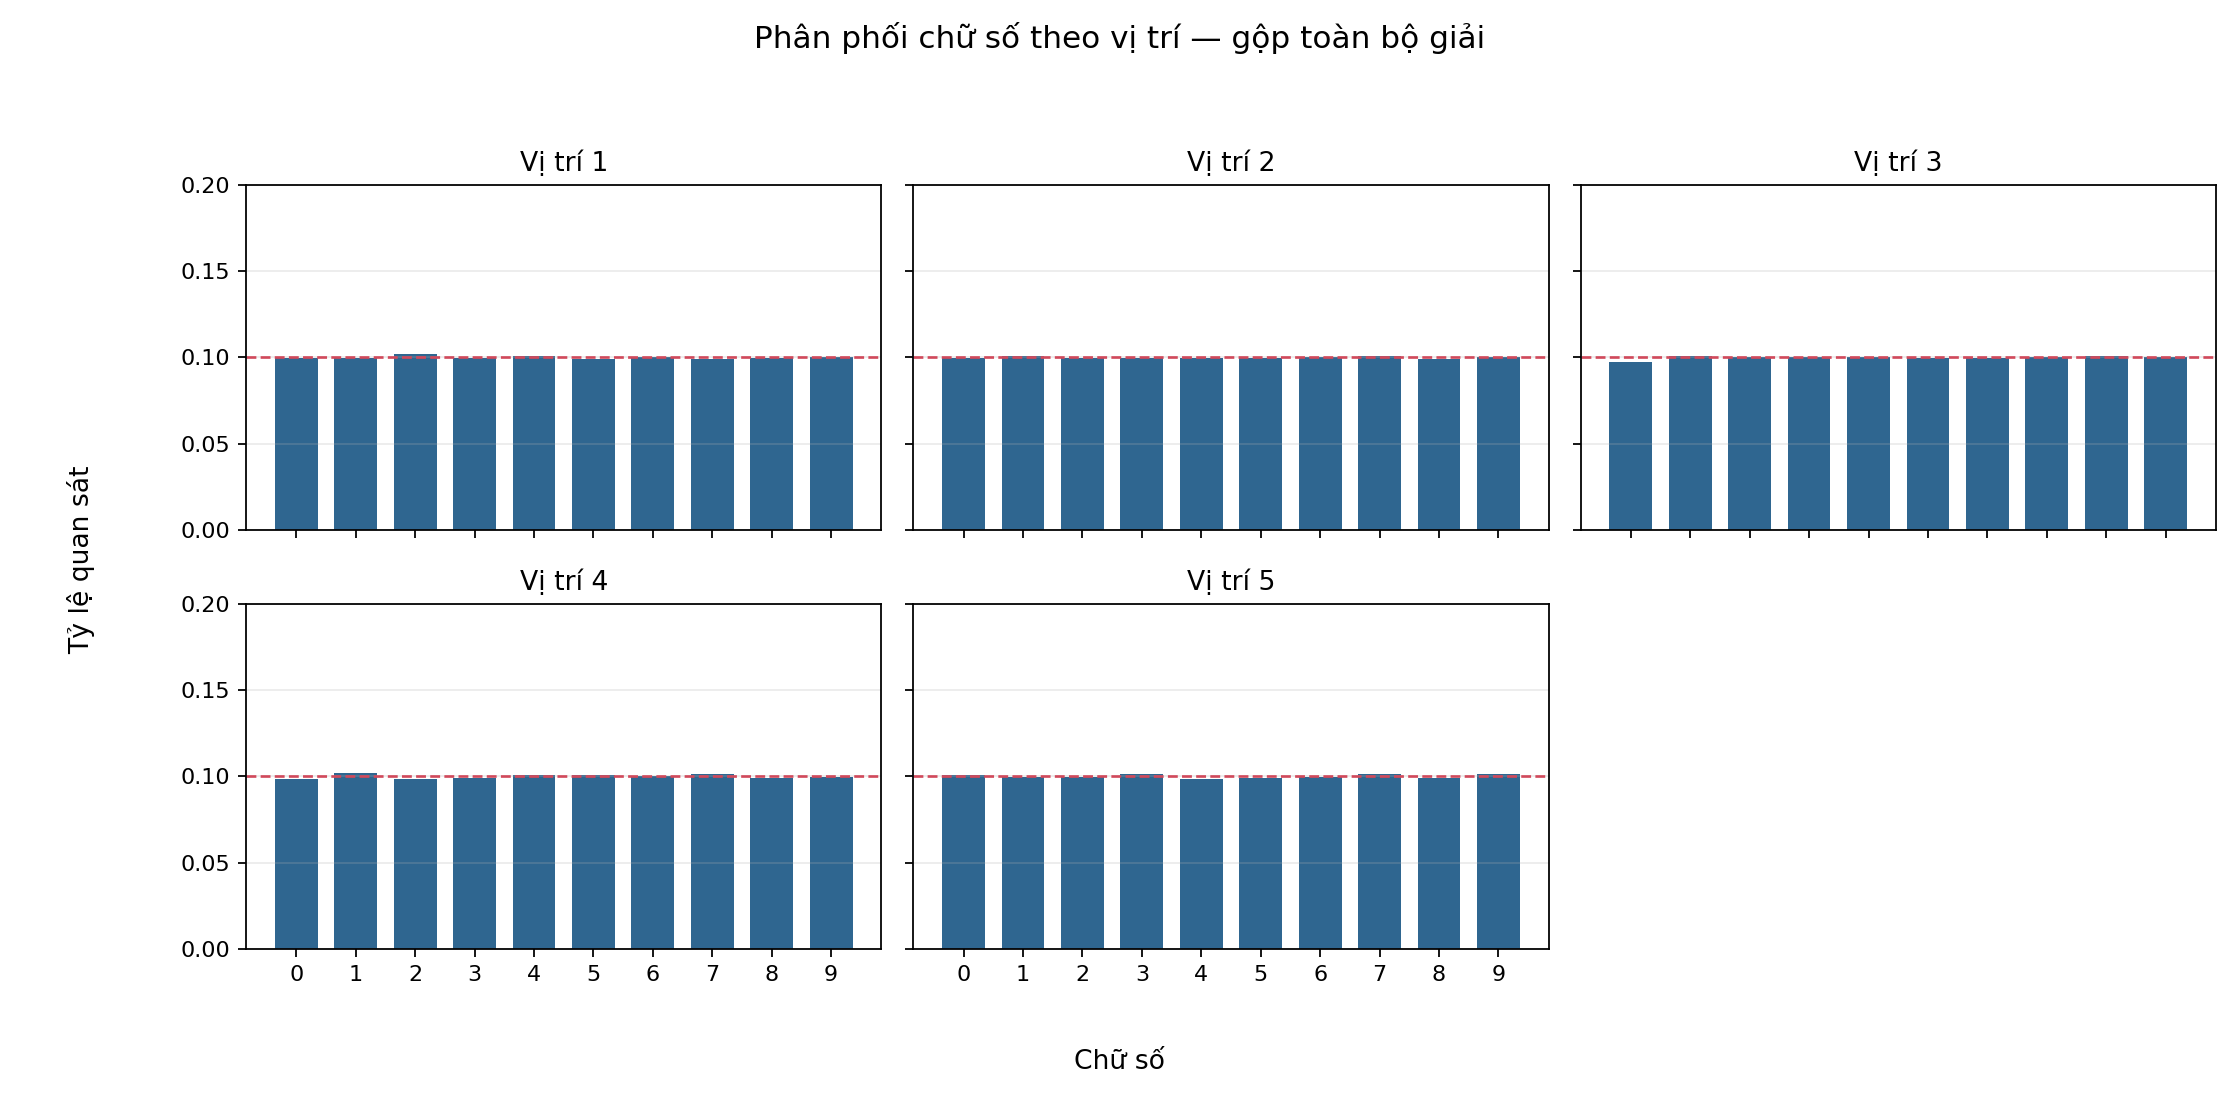
\includegraphics[width=0.92\linewidth]{../artifacts/p1_statistical_tests/01_digit_distribution/figures/01_pooled_digit_distribution.png}\caption{Phân phối chữ số theo vị trí trong toàn bộ dữ liệu.}\label{fig:p1-digit}\end{figure}

\section{Độc lập giữa các vị trí}
Kiểm định độc lập và thống kê liên hợp được dùng để xem chữ số ở các vị trí có liên hệ vượt quá mức kỳ vọng hay không. Không có bác bỏ nào trong 90 kiểm định sau FDR. Hình~\ref{fig:p1-position} trực quan hóa mức phụ thuộc rất nhỏ giữa các vị trí.
\begin{figure}[H]\centering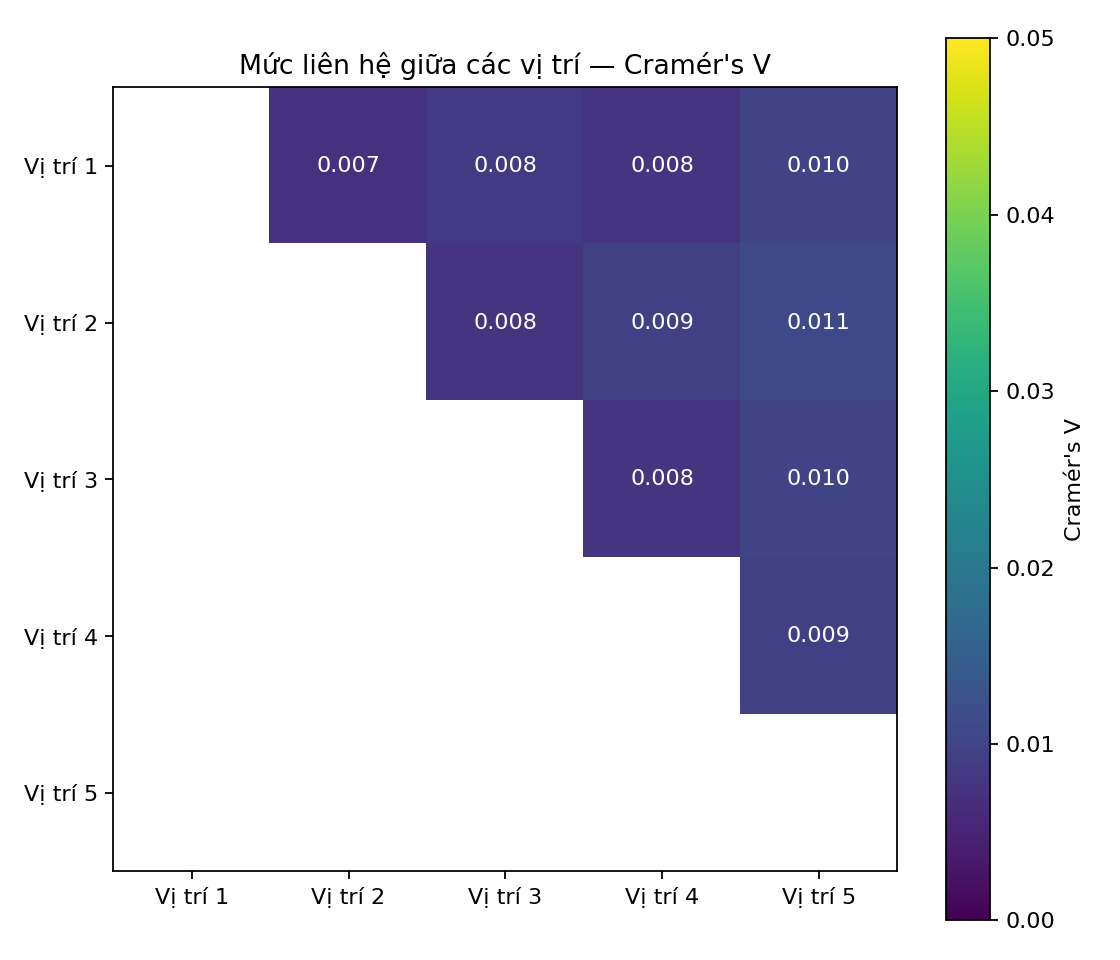
\includegraphics[width=0.92\linewidth]{../artifacts/p1_statistical_tests/02_position_independence/figures/02_pooled_position_dependence.png}\caption{Mức phụ thuộc giữa các vị trí chữ số.}\label{fig:p1-position}\end{figure}

\section{Phụ thuộc Markov và phụ thuộc theo độ trễ}
P1 kiểm tra cả phụ thuộc chuyển trạng thái ở lag 1 và phụ thuộc giữa các ngày ở lag 1--30. Không có kiểm định Markov nào trong 90 kiểm định bị bác bỏ; hình~\ref{fig:p1-markov} cho thấy độ lệch chuyển trạng thái không tạo cấu trúc nổi bật. Tương tự, thống kê Cramér's V theo các độ trễ không cho thấy tín hiệu bền vững (Hình~\ref{fig:p1-lag}).
\begin{figure}[H]\centering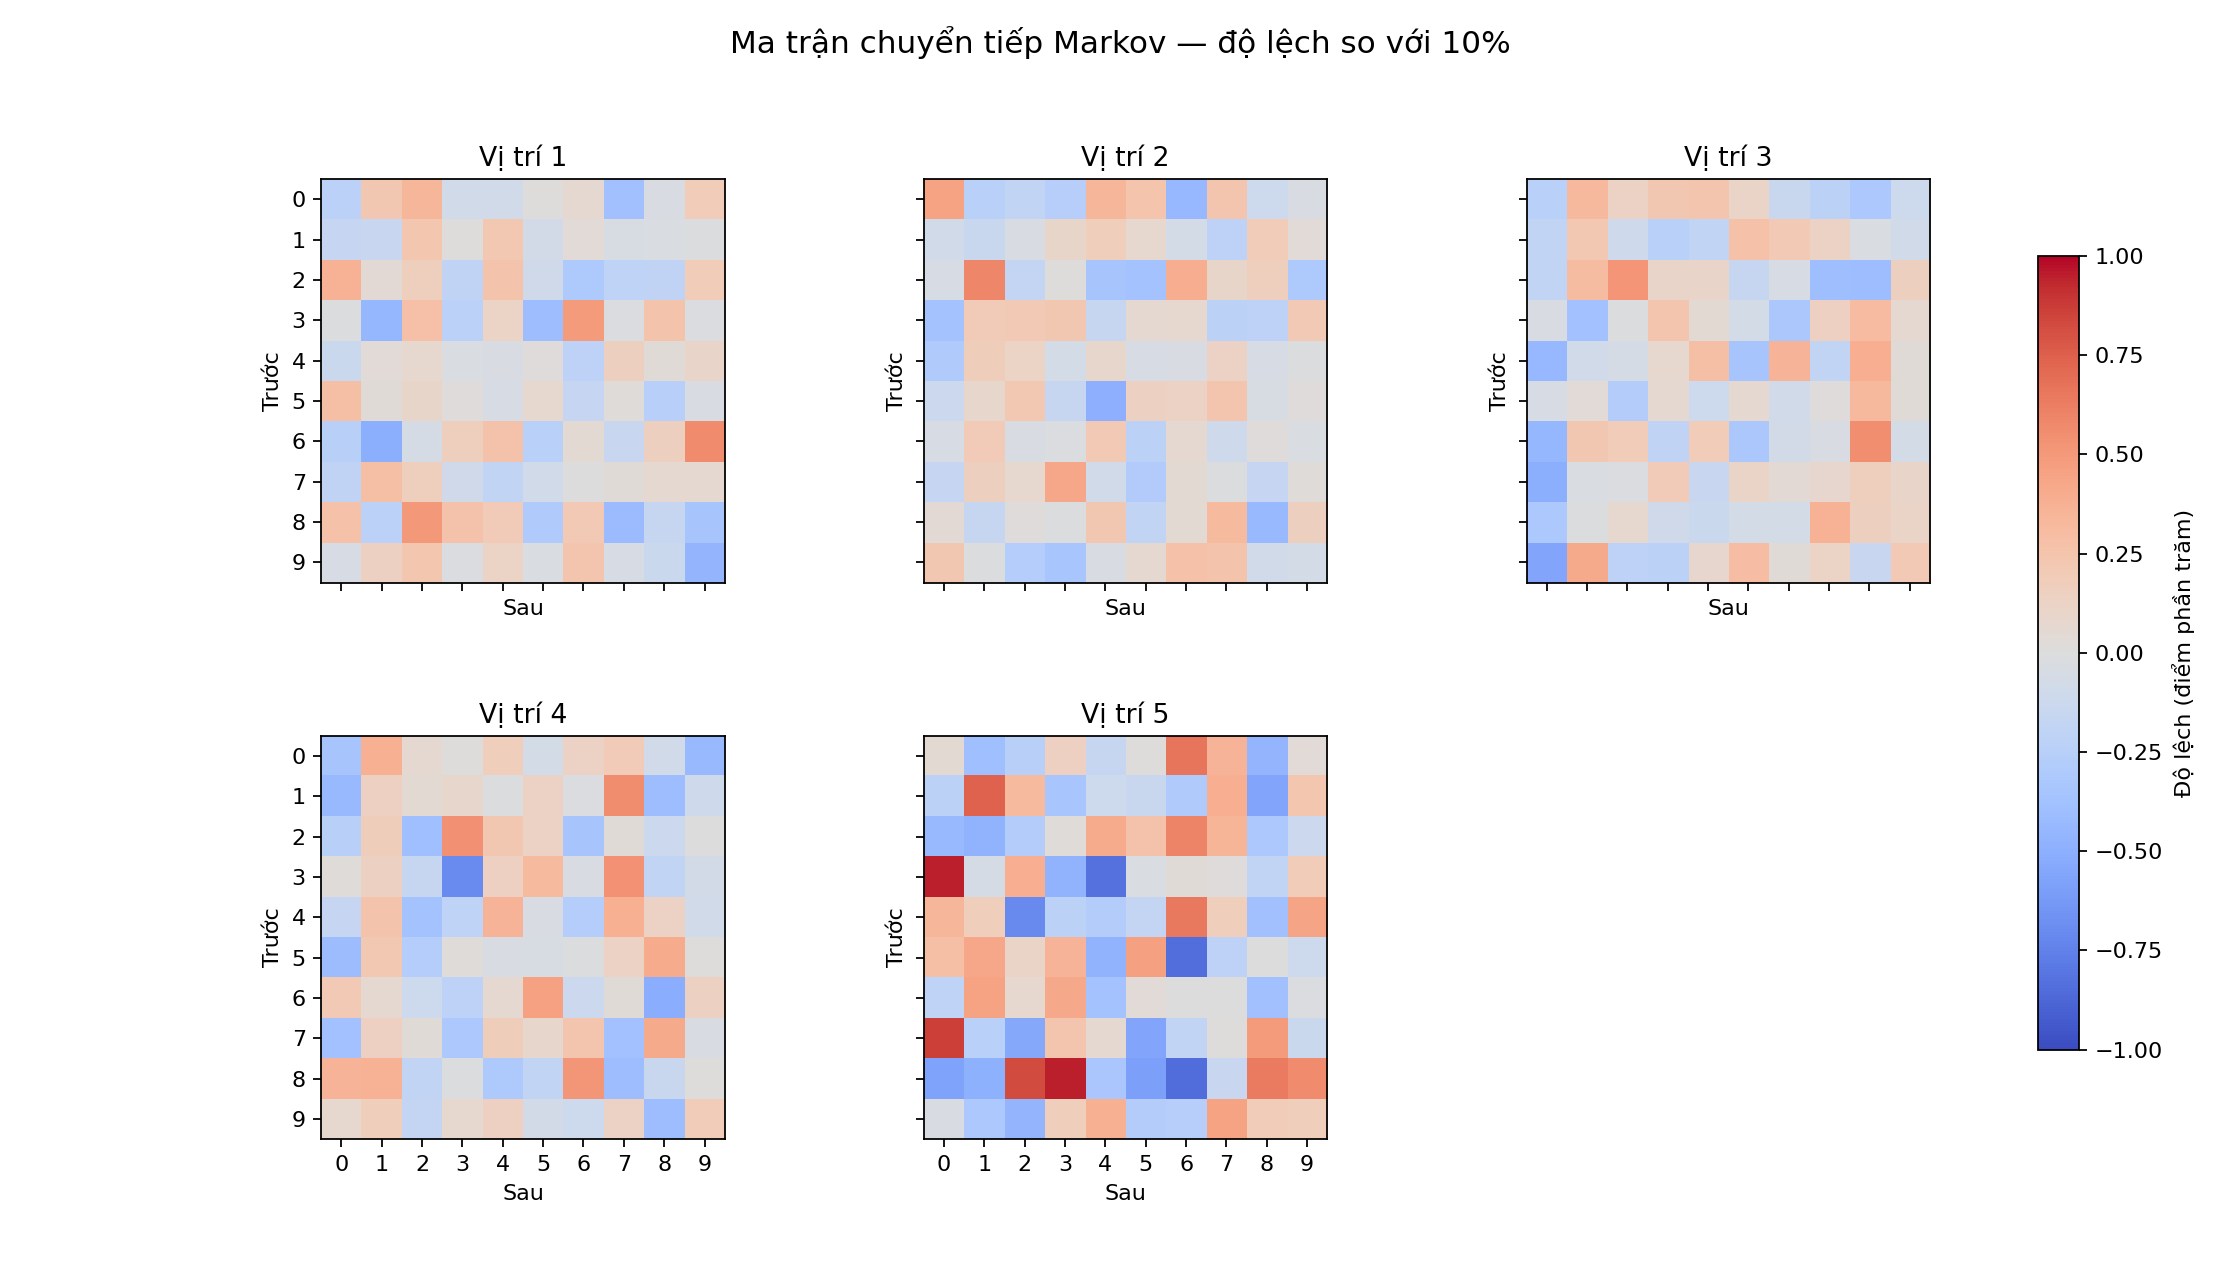
\includegraphics[width=0.92\linewidth]{../artifacts/p1_statistical_tests/03_markov_by_position/figures/01_transition_deviations.png}\caption{Độ lệch của ma trận chuyển trạng thái Markov lag 1.}\label{fig:p1-markov}\end{figure}
\begin{figure}[H]\centering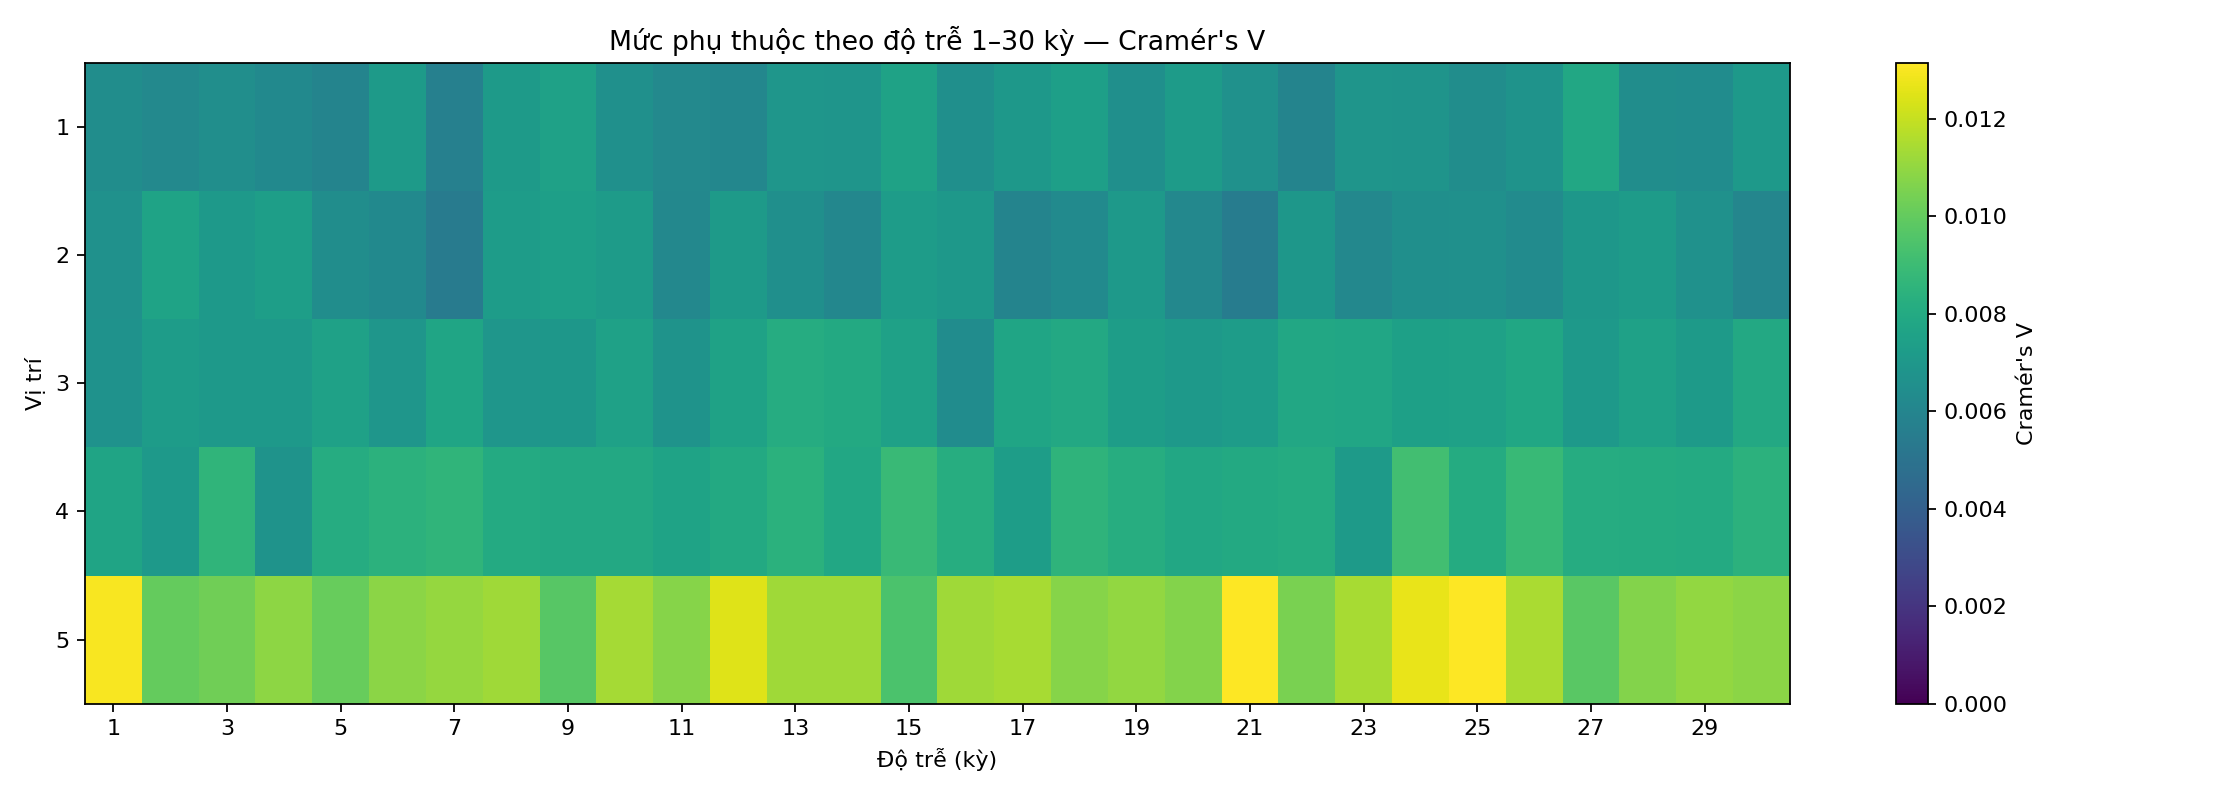
\includegraphics[width=0.92\linewidth]{../artifacts/p1_statistical_tests/04_temporal_randomness/figures/04_lag_dependence_cramers_v.png}\caption{Phụ thuộc theo độ trễ 1--30 ngày bằng Cramér's V.}\label{fig:p1-lag}\end{figure}

\section{Ổn định theo thời gian và trúng đồng thời}
Phân tích ổn định chia chuỗi theo giai đoạn và lặp lại các kiểm định chính. Không có bác bỏ nào trong 4050 kiểm định; Hình~\ref{fig:p1-stability} tóm tắt kết quả ý nghĩa theo từng nhóm. Tỷ lệ ngày có ít nhất hai giải cùng chứa một đuôi số là 62,63\%; ít nhất ba giải là 0,25\%; ít nhất bốn giải xấp xỉ 0,00\%. Đây là mô tả cơ chế chồng lấn của nhiều giải, không phải bằng chứng dự báo.
\begin{figure}[H]\centering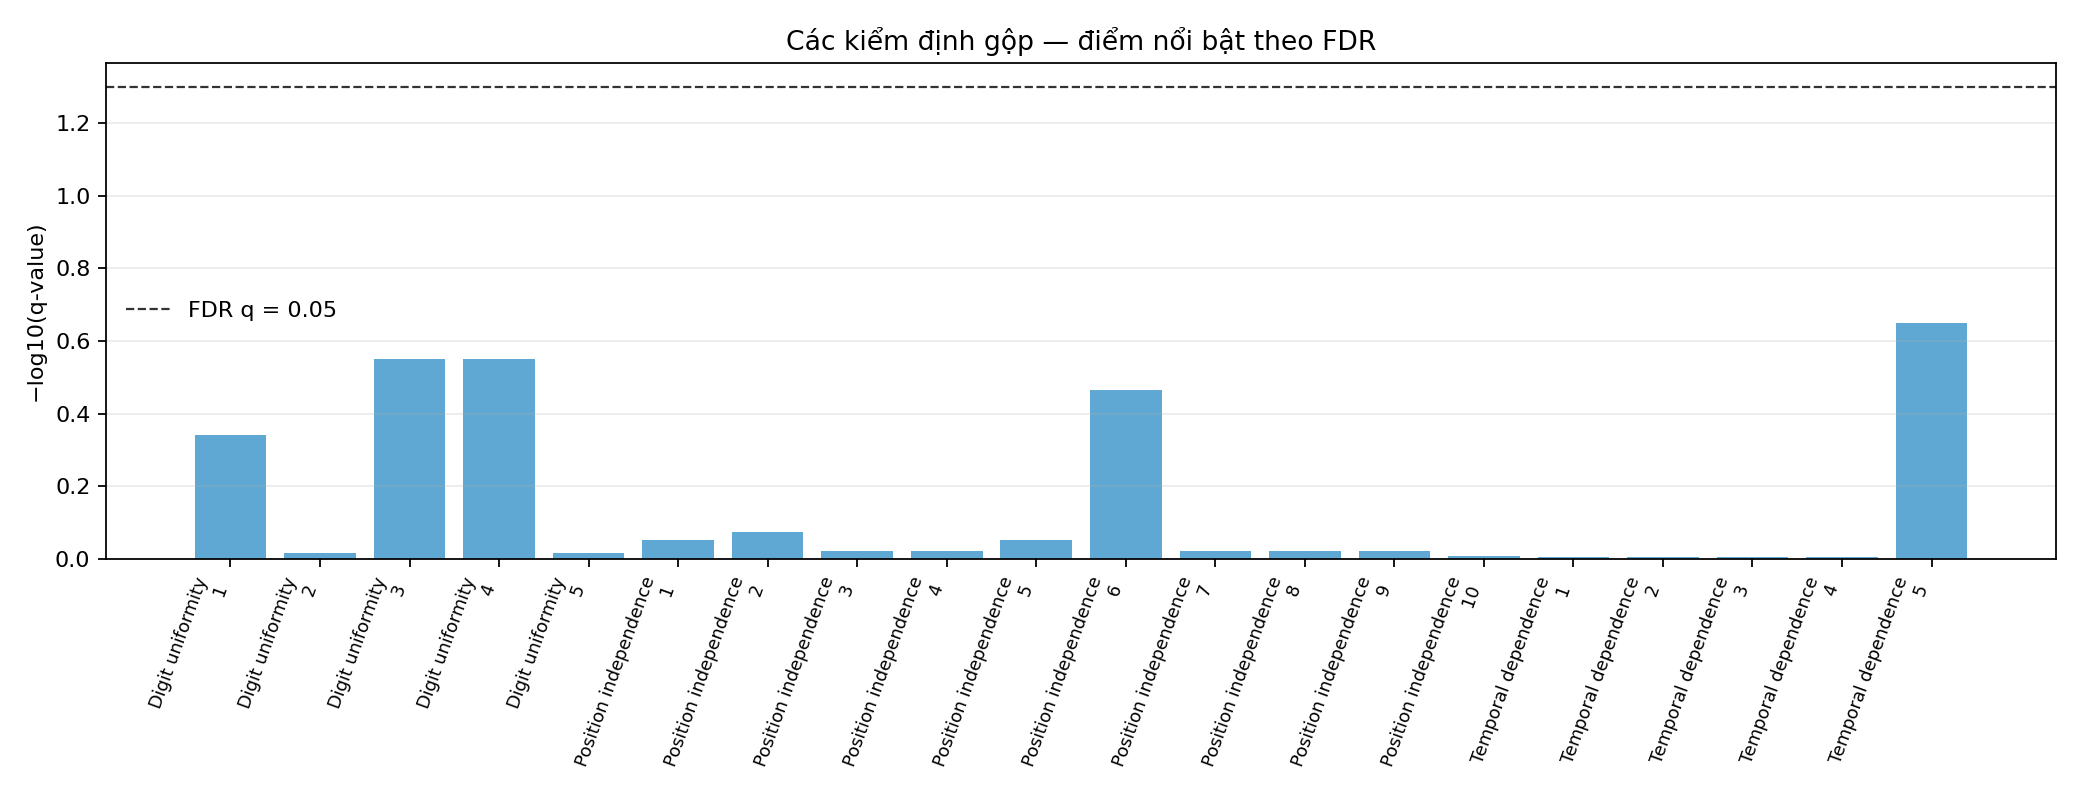
\includegraphics[width=0.92\linewidth]{../artifacts/p1_statistical_tests/04b_temporal_stability/figures/04_pooled_test_significance.png}\caption{Kết quả kiểm định gộp trong phân tích ổn định theo thời gian.}\label{fig:p1-significance}\end{figure}
\begin{figure}[H]\centering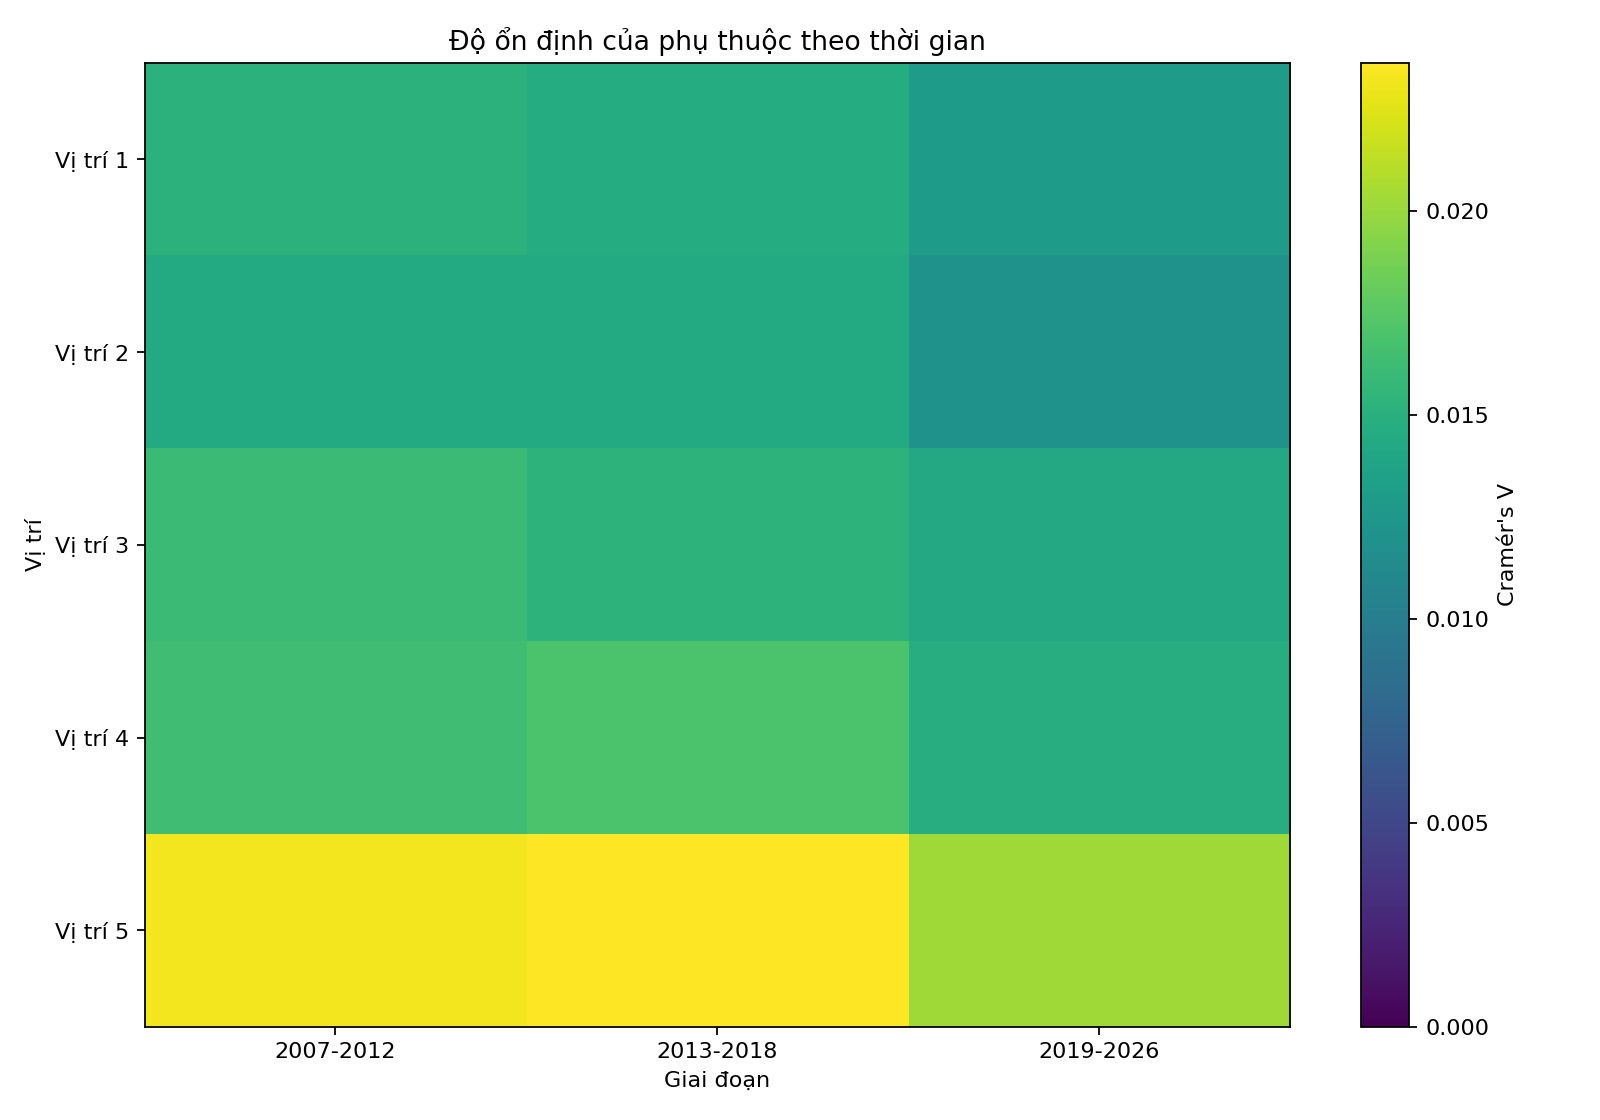
\includegraphics[width=0.92\linewidth]{../artifacts/p1_statistical_tests/04b_temporal_stability/figures/05_temporal_stability.png}\caption{Độ ổn định của các thống kê theo giai đoạn.}\label{fig:p1-stability}\end{figure}
\begin{figure}[H]\centering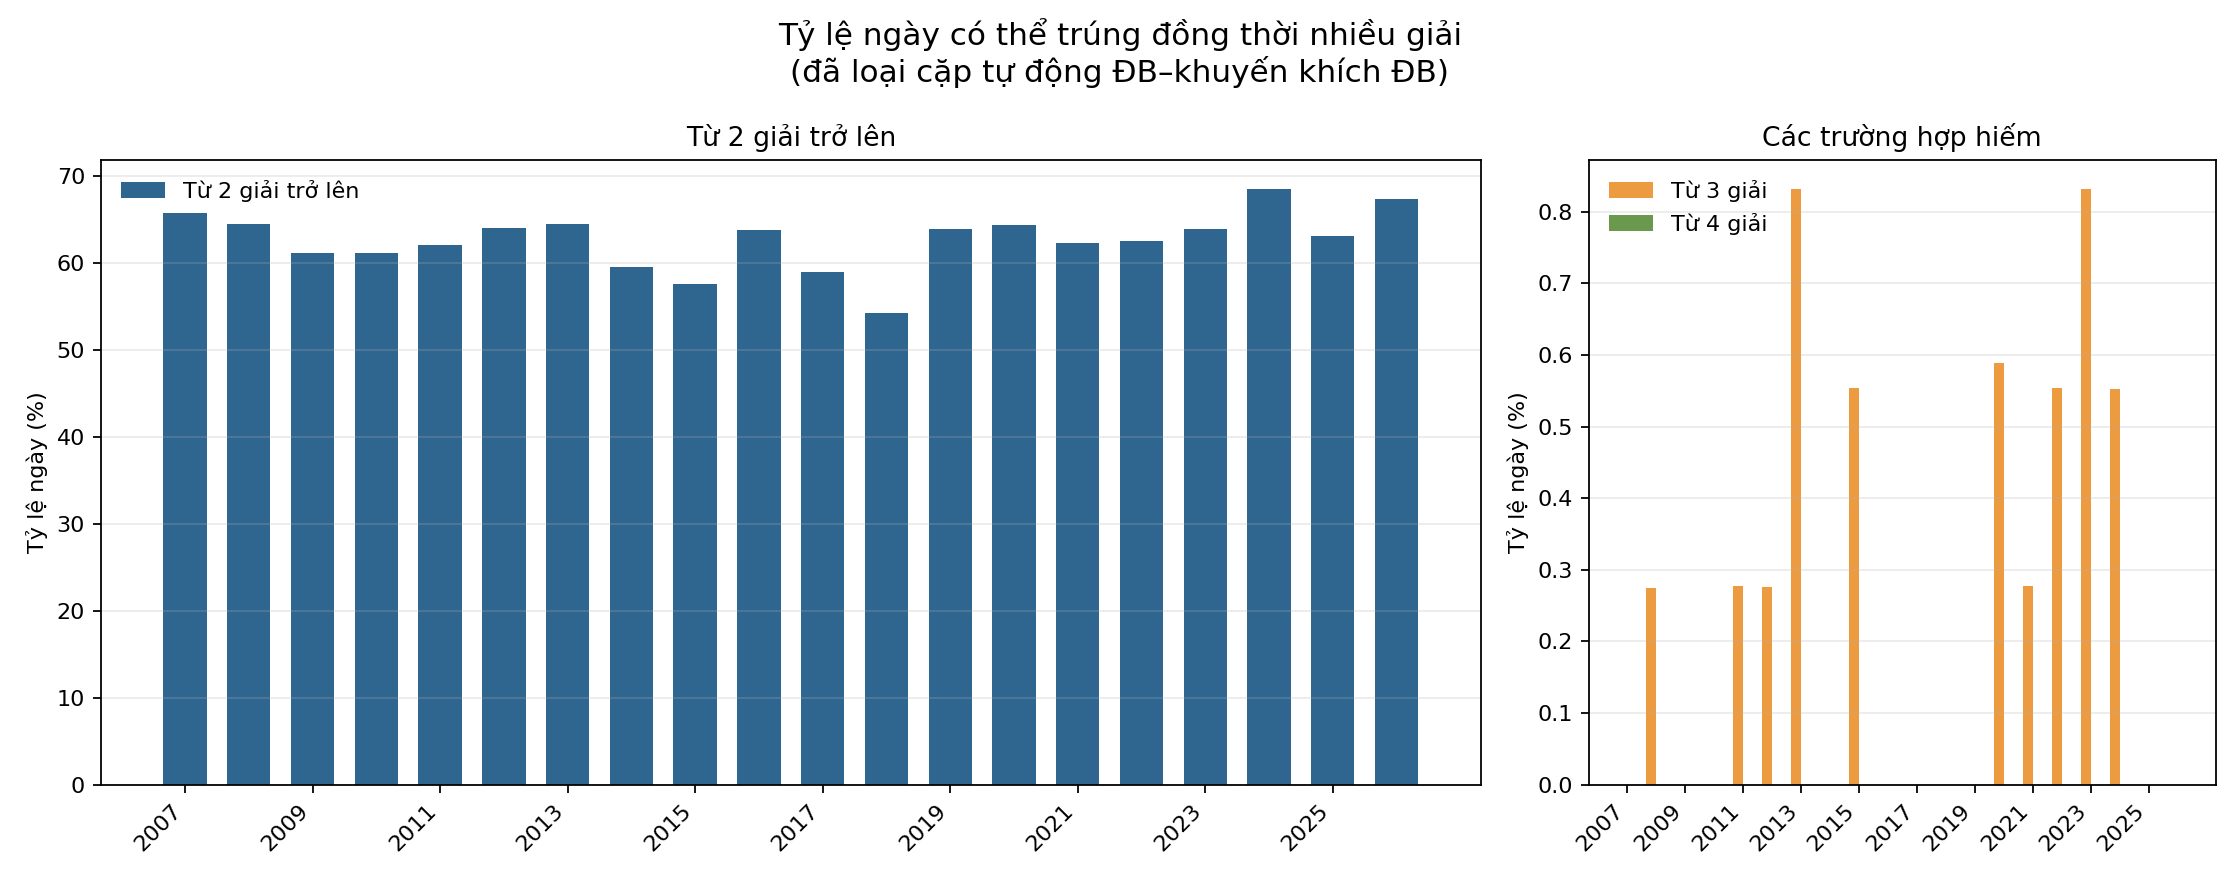
\includegraphics[width=0.92\linewidth]{../artifacts/p1_statistical_tests/04_temporal_randomness/figures/03_multi_win_rates_by_year.png}\caption{Tỷ lệ trúng đồng thời nhiều giải theo năm.}\label{fig:p1-multi}\end{figure}

\section{Kết luận P1}
Các kiểm định cung cấp bằng chứng nhất quán với một quá trình gần ngẫu nhiên ở mức độ cần thiết cho dự báo thực hành. Một vài sai lệch cục bộ có thể xuất hiện do kích thước mẫu lớn, do cơ chế nhiều giải trong cùng ngày hoặc do biến thiên ngẫu nhiên. Vì vậy, P1 chỉ cho phép chuyển sang kiểm tra dự báo ngoài mẫu; không cho phép khẳng định có lợi thế chơi.

\chapter{MÔ HÌNH DỰ BÁO CHỮ SỐ}
\section{Biến mục tiêu}
Với mỗi vị trí và chữ số, mục tiêu bằng 1 nếu chữ số xuất hiện trong ít nhất một của 27 kết quả trong ngày, bằng 0 nếu không xuất hiện. Đây là bài toán phân loại nhị phân nhiều đầu ra, khác với đoán chính xác một số duy nhất từ 00 đến 99.

\section{Mô hình}
Đường cơ sở là Uniform. Nhóm xác suất gồm CDM/Dirichlet-Multinomial, Rolling CDM và Bayesian Markov; nhóm học máy gồm CatBoost và XGBoost. Các mô hình được đánh giá theo walk-forward, trong đó dữ liệu của ngày hiện tại chỉ được đưa vào trạng thái sau khi dự báo đã hoàn tất.

Đối với bài toán pool, xác suất được ước lượng riêng cho năm vị trí và mười chữ số. Đối với bài toán giải, mô hình dự báo xác suất của số năm chữ số theo từng nhóm giải. Hai bài toán được báo cáo riêng vì pool có thể hỗ trợ xây dựng vé, nhưng không đồng nghĩa với xác suất một vé cụ thể trúng giải cao.

\begin{table}[H]\centering
\caption{Kết quả validation 2023--2024}
\begin{tabular}{lrr}\toprule
Mô hình & Brier score & Log loss\\\midrule
Expanding Beta & 0.097820 & 0.329968\\
Markov presence & 0.097853 & 0.330118\\
Rolling Beta 365 & 0.097973 & 0.330935\\
CatBoost & 0.098313 & 0.332414\\
Random Forest & 0.098615 & 0.333515\\
XGBoost & 0.099221 & 0.336660\\
Rolling Beta 90 & 0.098779 & 0.335109\\
Rolling Beta 30 & 0.100920 & 0.343546\\
Dirichlet daily & 0.112701 & 0.397621\\
Uniform 27-IID & 0.113875 & 0.408108\\\bottomrule
\end{tabular}\end{table}

Expanding Beta tốt nhất trên validation theo Brier score và log loss trong bảng benchmark hiện có. CatBoost là mô hình học máy tốt nhất nhưng chưa vượt nhóm Bayesian/Markov. Trên final test 2025--2026, Expanding Beta đạt Brier 0.104579 và log loss 0.351395; Uniform lần lượt 0.104588 và 0.351453, chênh lệch rất nhỏ. Kết quả này chỉ phản ánh mục tiêu pool theo ngày, không được suy diễn thành khả năng đoán chính xác giải Đặc biệt.

\chapter{CHIẾN LƯỢC VÀ BACKTEST}
\section{Thiết kế chiến lược}
P3 chuyển xác suất chữ số thành các pool năm vị trí, rồi sinh vé bằng tích Descartes. Ba cấu hình được kiểm thử là $2\times2\times2\times2\times2=32$ vé, $3\times2\times2\times2\times1=24$ vé và $3\times3\times2\times1\times1=18$ vé mỗi ngày. Một nhánh riêng tập trung vào giải Bảy: chọn các tiền tố đứng đầu ở ba vị trí đầu và thử $m=1,\ldots,10$ đuôi số đứng đầu ở hai vị trí cuối.

Mỗi vé có giá 10.000 VND. Kết quả được đối sánh với toàn bộ 27 giải năm chữ số trong ngày; một vé có thể nhận nhiều giải hợp lệ. Mức trả trong code backtest là: Phụ Đặc biệt 25.000.000; Khuyến khích Đặc biệt 40.000; giải Nhất 10.000.000; Nhì 5.000.000; Ba 1.000.000; Tư 400.000; Năm 200.000; Sáu 100.000; Bảy 40.000 VND.

\section{Chia tập và chỉ số}
Validation 2023--2024 dùng để so sánh ứng viên; final test 2025--2026 chỉ được mở một lần cho đánh giá cuối. Lợi nhuận ngày là
\[
\Pi_t=\sum_{g\in G_t}R_g-10\,000 n_t,
\]
trong đó $G_t$ là tập giải vé nhận được, $R_g$ là tiền trả của giải và $n_t$ là số vé. ROI bằng tổng lợi nhuận chia tổng chi phí. Cách tính này tránh áp dụng một công thức hòa vốn duy nhất cho các chiến lược có cơ cấu giải khác nhau.

\section{Kết quả P3}
\begin{table}[H]\centering\small
\caption{Backtest các cấu hình pool năm chữ số}\label{tab:p3-summary}
\begin{tabular}{llrrrr}\toprule
Fold & Cấu hình & Số ngày & Số vé & Lợi nhuận (VND) & ROI\\\midrule
Validation & 32 vé & 723 & 23136 & -143.600.000 & -62,07\%\\
Validation & 24 vé & 723 & 17352 & -134.120.000 & -77,29\%\\
Validation & 18 vé & 723 & 13014 & -104.580.000 & -80,36\%\\
Final test & 32 vé & 606 & 19392 & -147.120.000 & -75,87\%\\
Final test & 24 vé & 606 & 14544 & -110.000.000 & -75,63\%\\
Final test & 18 vé & 606 & 10908 & -86.940.000 & -79,70\%\\\bottomrule
\end{tabular}\end{table}

\begin{figure}[H]\centering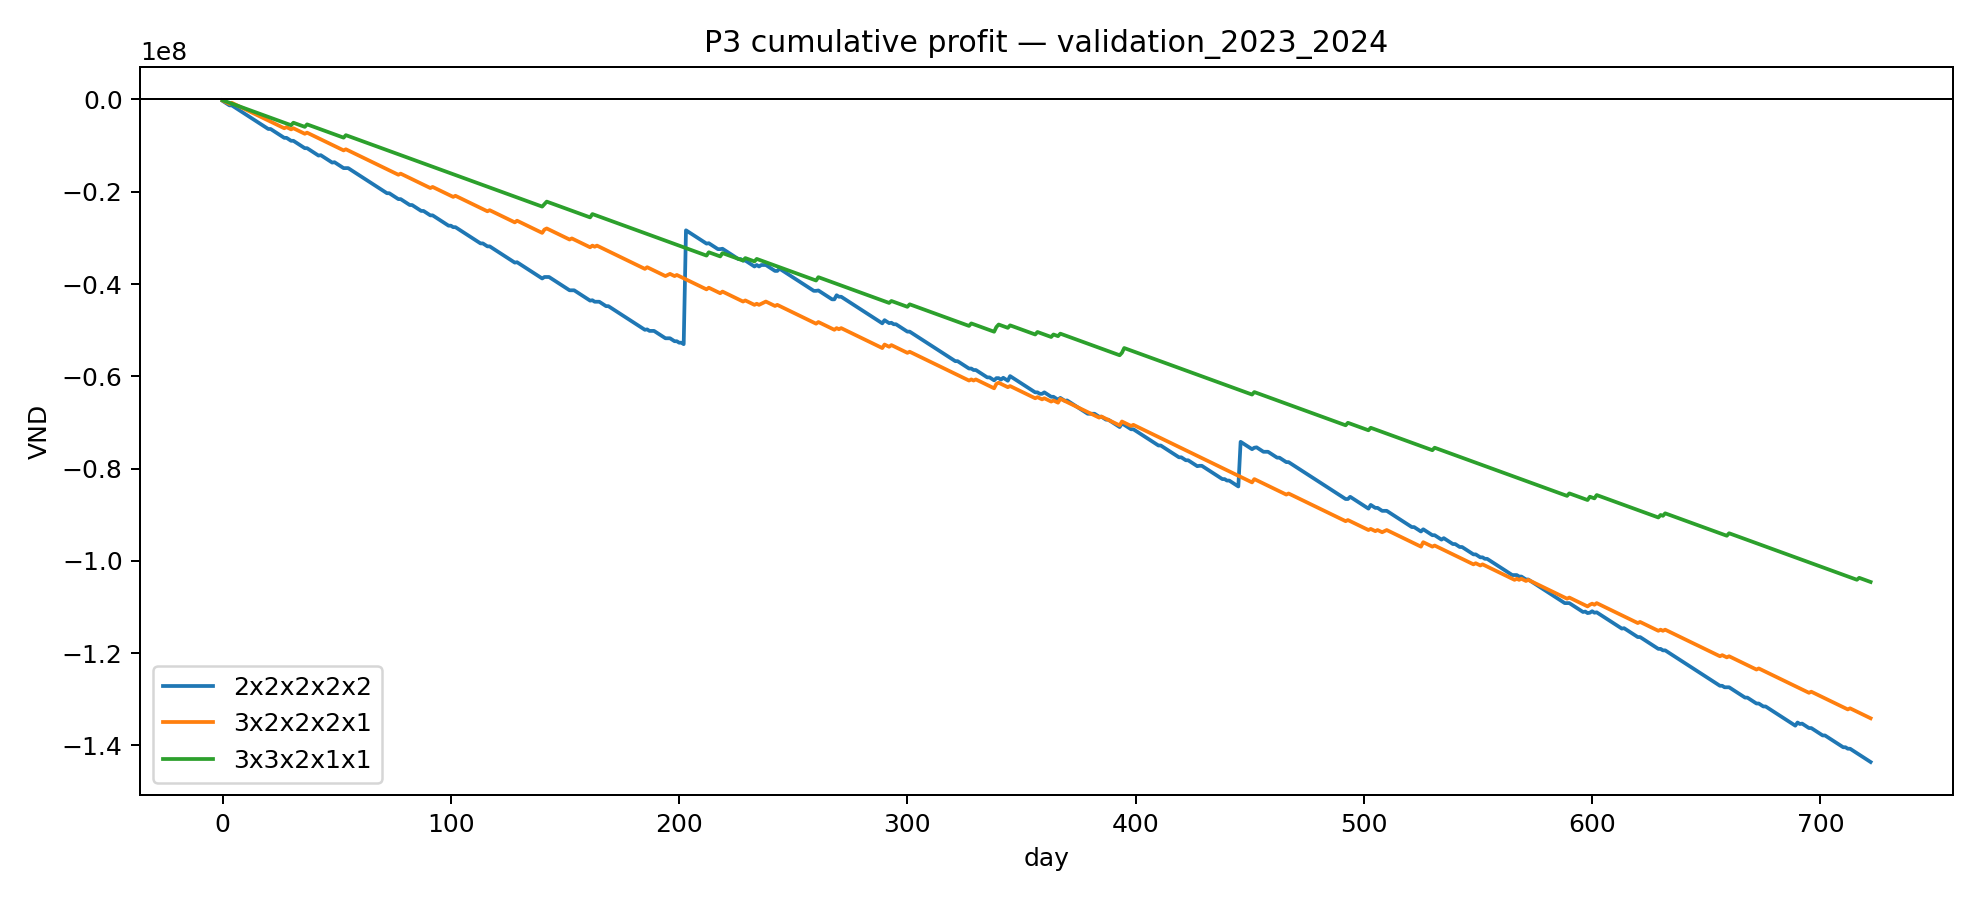
\includegraphics[width=0.92\linewidth]{../artifacts/p3_strategies/cumulative_profit_validation_2023_2024.png}\caption{Lợi nhuận tích lũy của các pool trên validation.}\end{figure}
\begin{figure}[H]\centering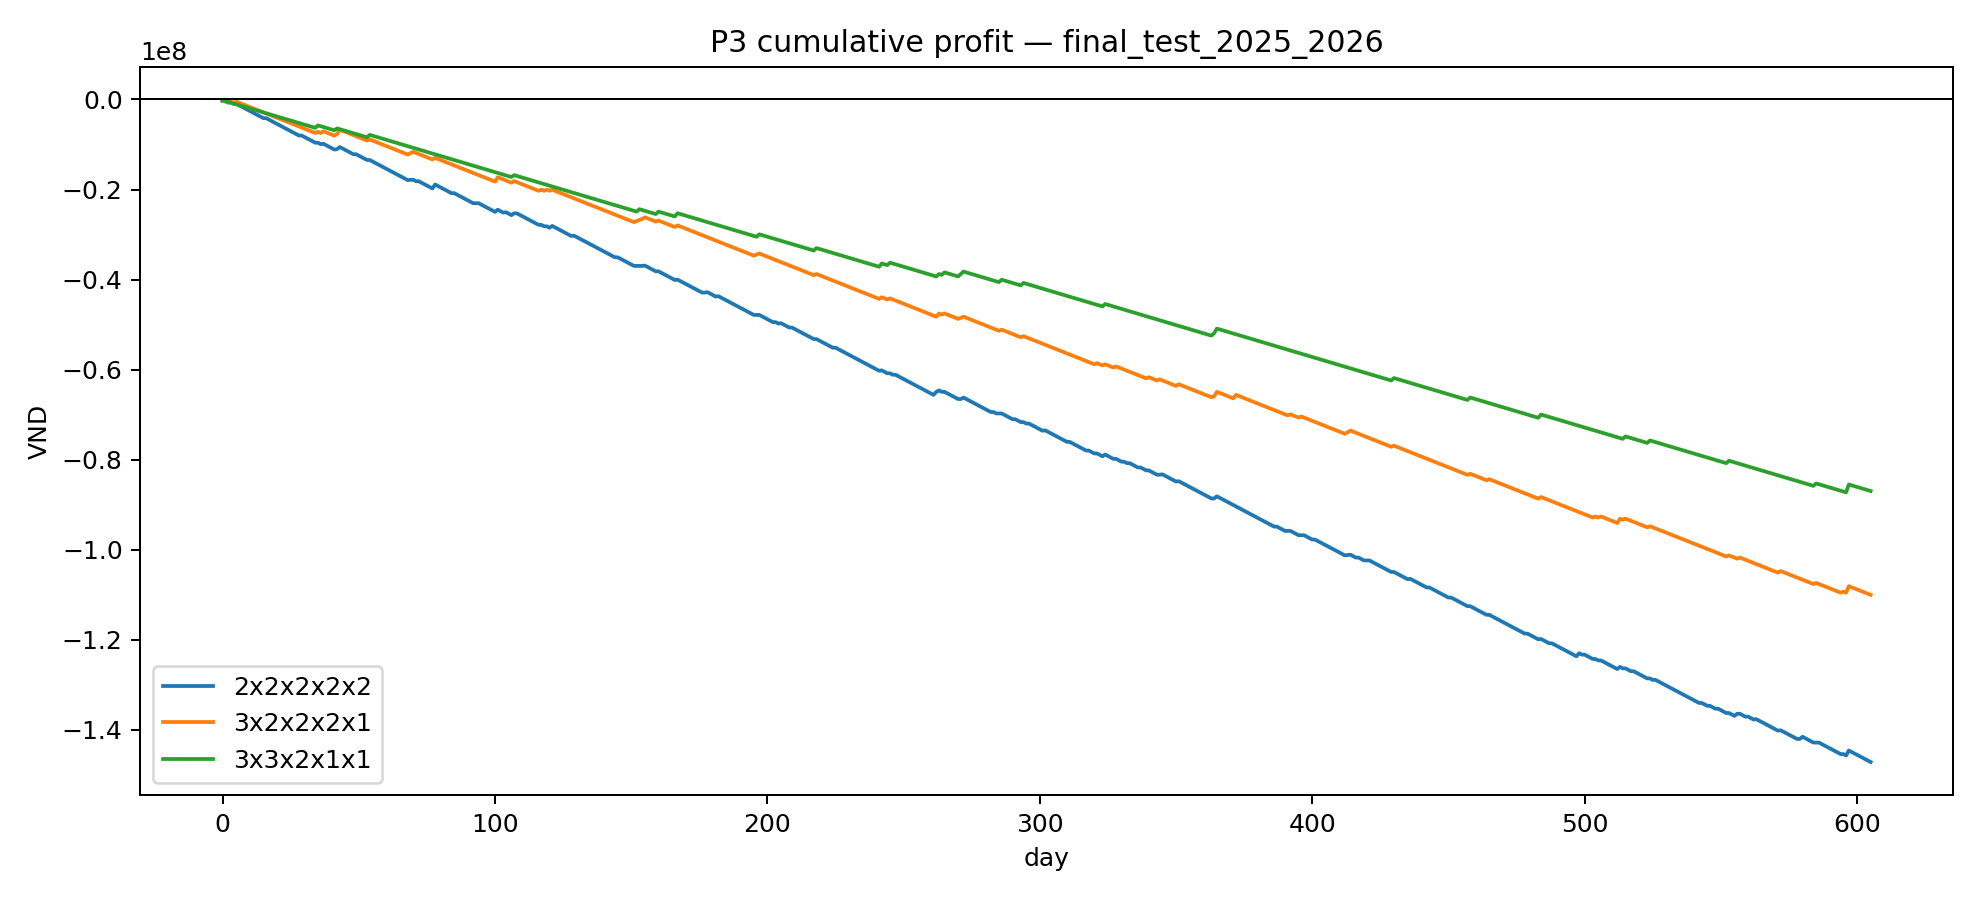
\includegraphics[width=0.92\linewidth]{../artifacts/p3_strategies/cumulative_profit_final_test_2025_2026.png}\caption{Lợi nhuận tích lũy của các pool trên final test.}\end{figure}

\section{Chiến lược giải Bảy theo $m$}
Kết quả theo $m$ được giữ lại như một thí nghiệm độ nhạy. Việc tăng $m$ làm tăng số lựa chọn và chi phí, nhưng không bảo đảm tăng lợi nhuận; do đó, cấu hình tốt nhất phải được khóa từ validation trước khi xem final test.
\begin{figure}[H]\centering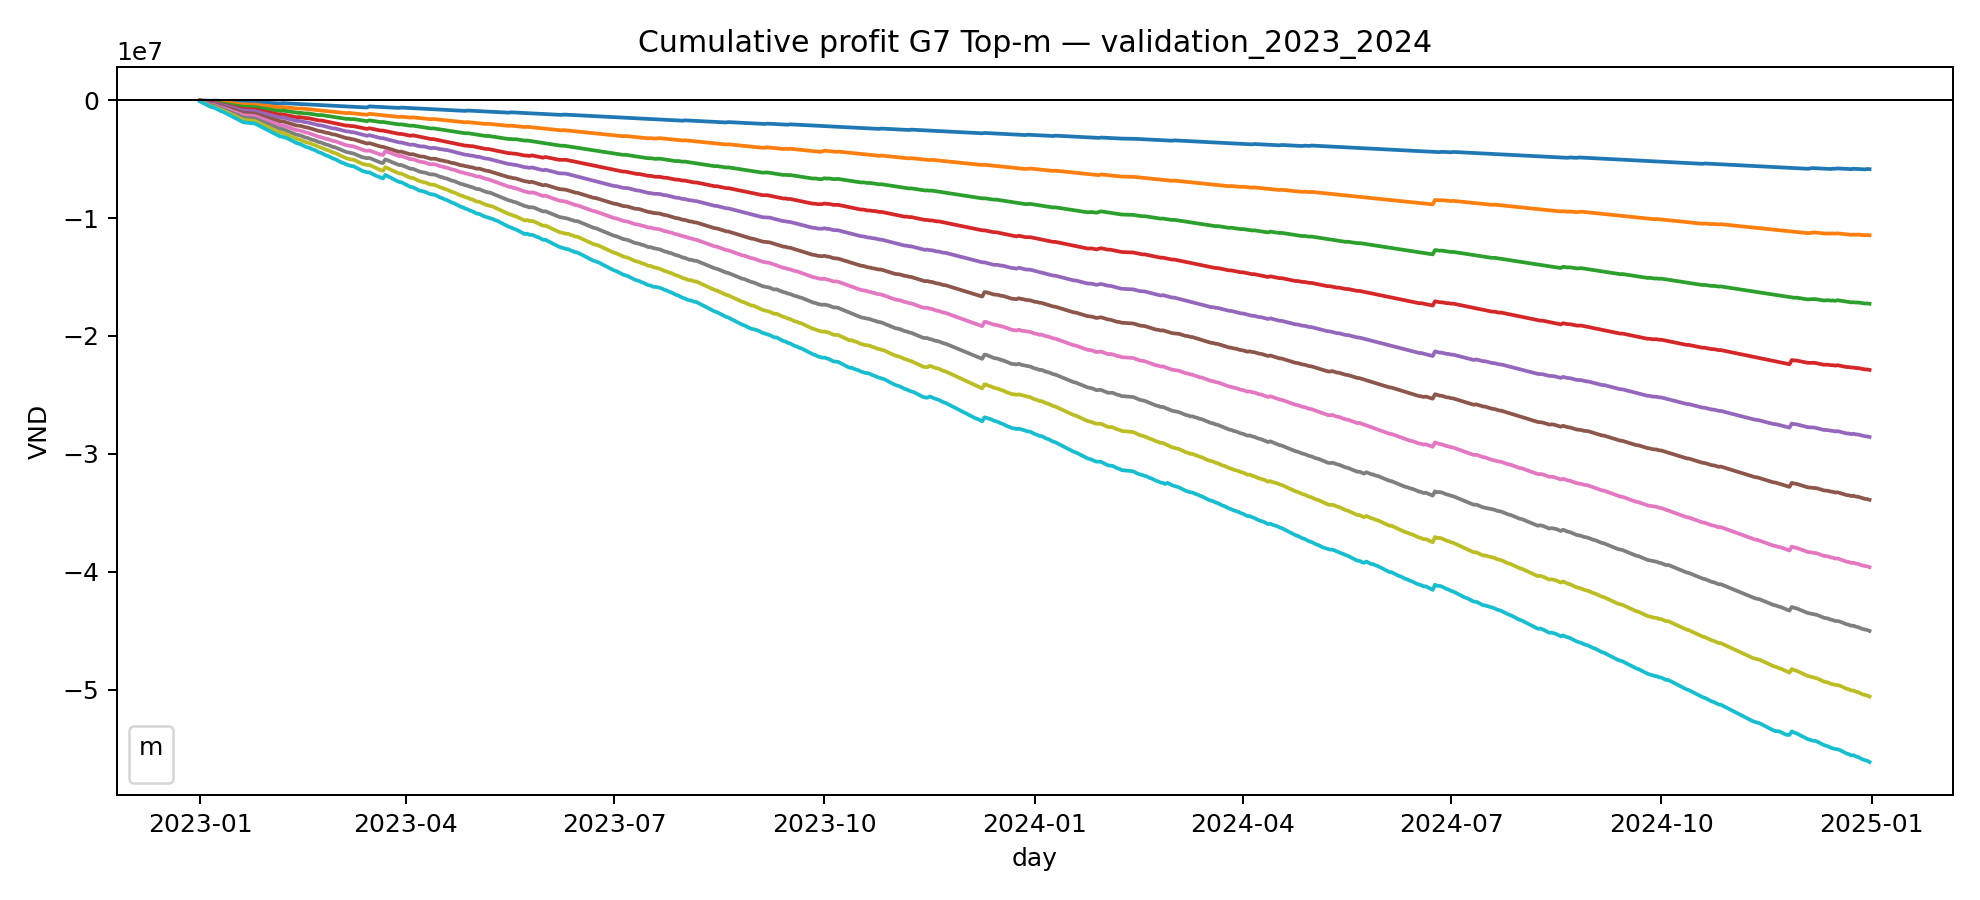
\includegraphics[width=0.92\linewidth]{../artifacts/p3_strategies/g7_topm_prefix/cumulative_profit_validation_2023_2024.png}\caption{Lợi nhuận tích lũy của chiến lược tập trung giải Bảy trên validation.}\end{figure}
\begin{figure}[H]\centering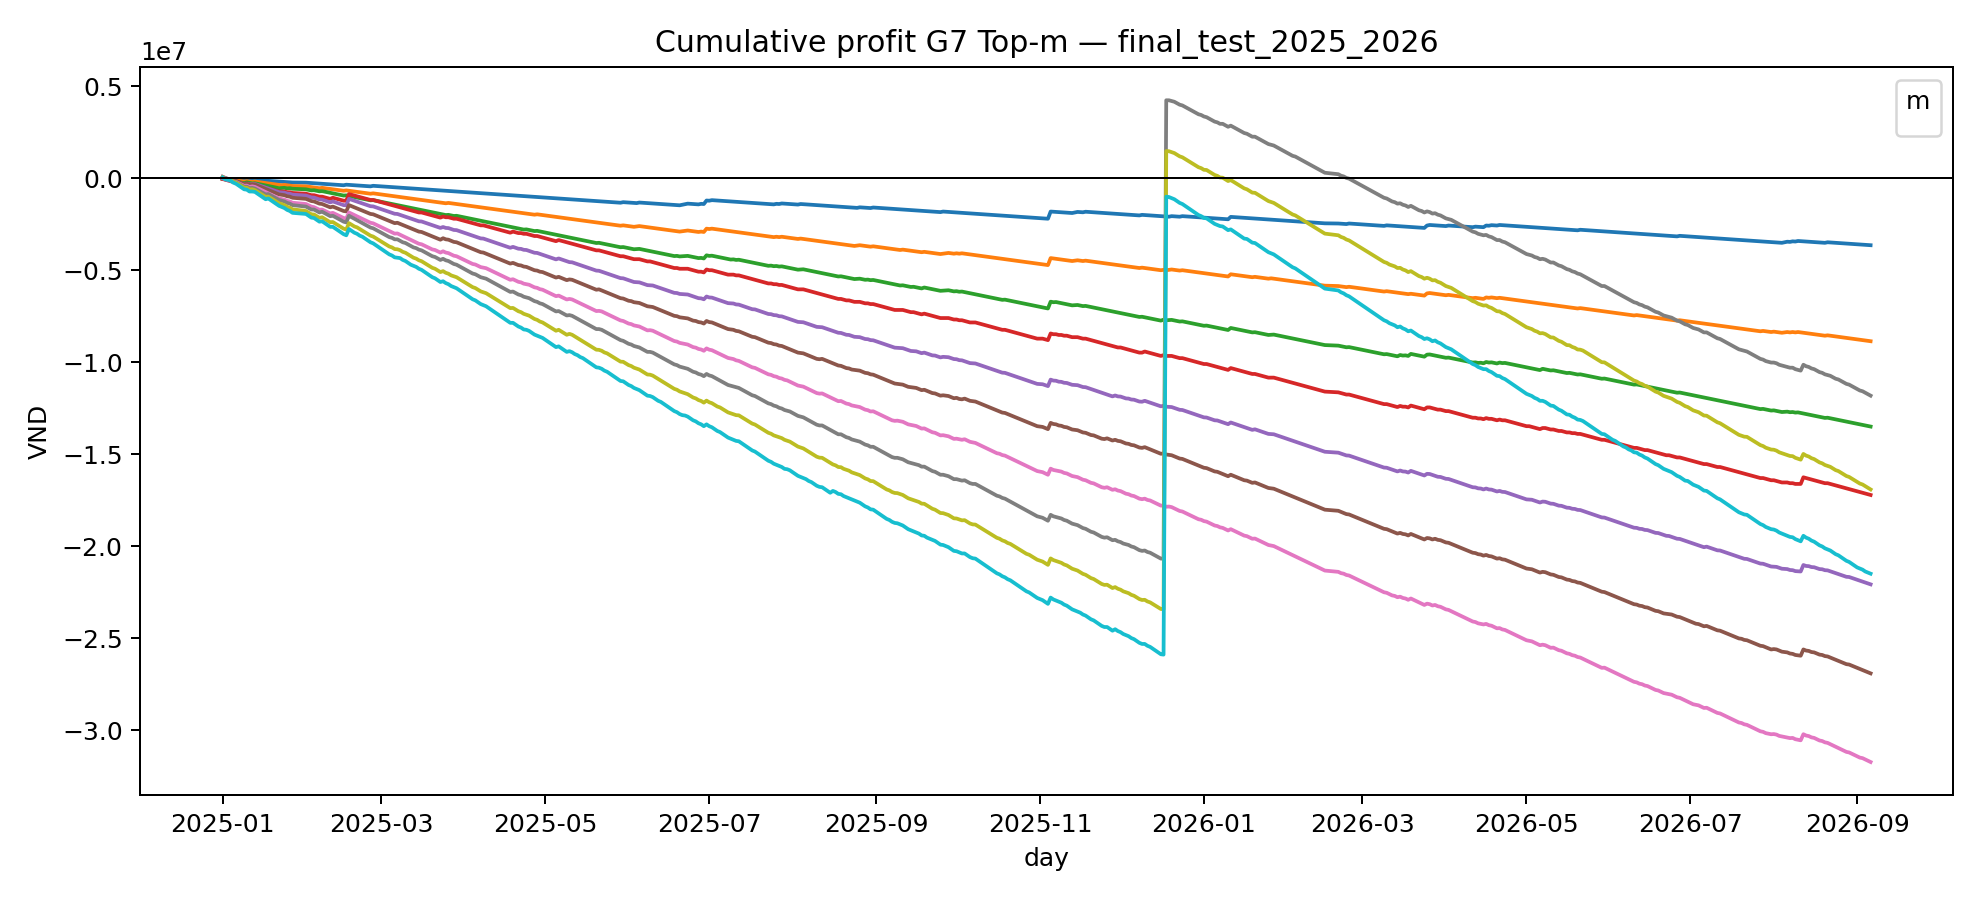
\includegraphics[width=0.92\linewidth]{../artifacts/p3_strategies/g7_topm_prefix/cumulative_profit_final_test_2025_2026.png}\caption{Lợi nhuận tích lũy của chiến lược tập trung giải Bảy trên final test.}\end{figure}
\begin{figure}[H]\centering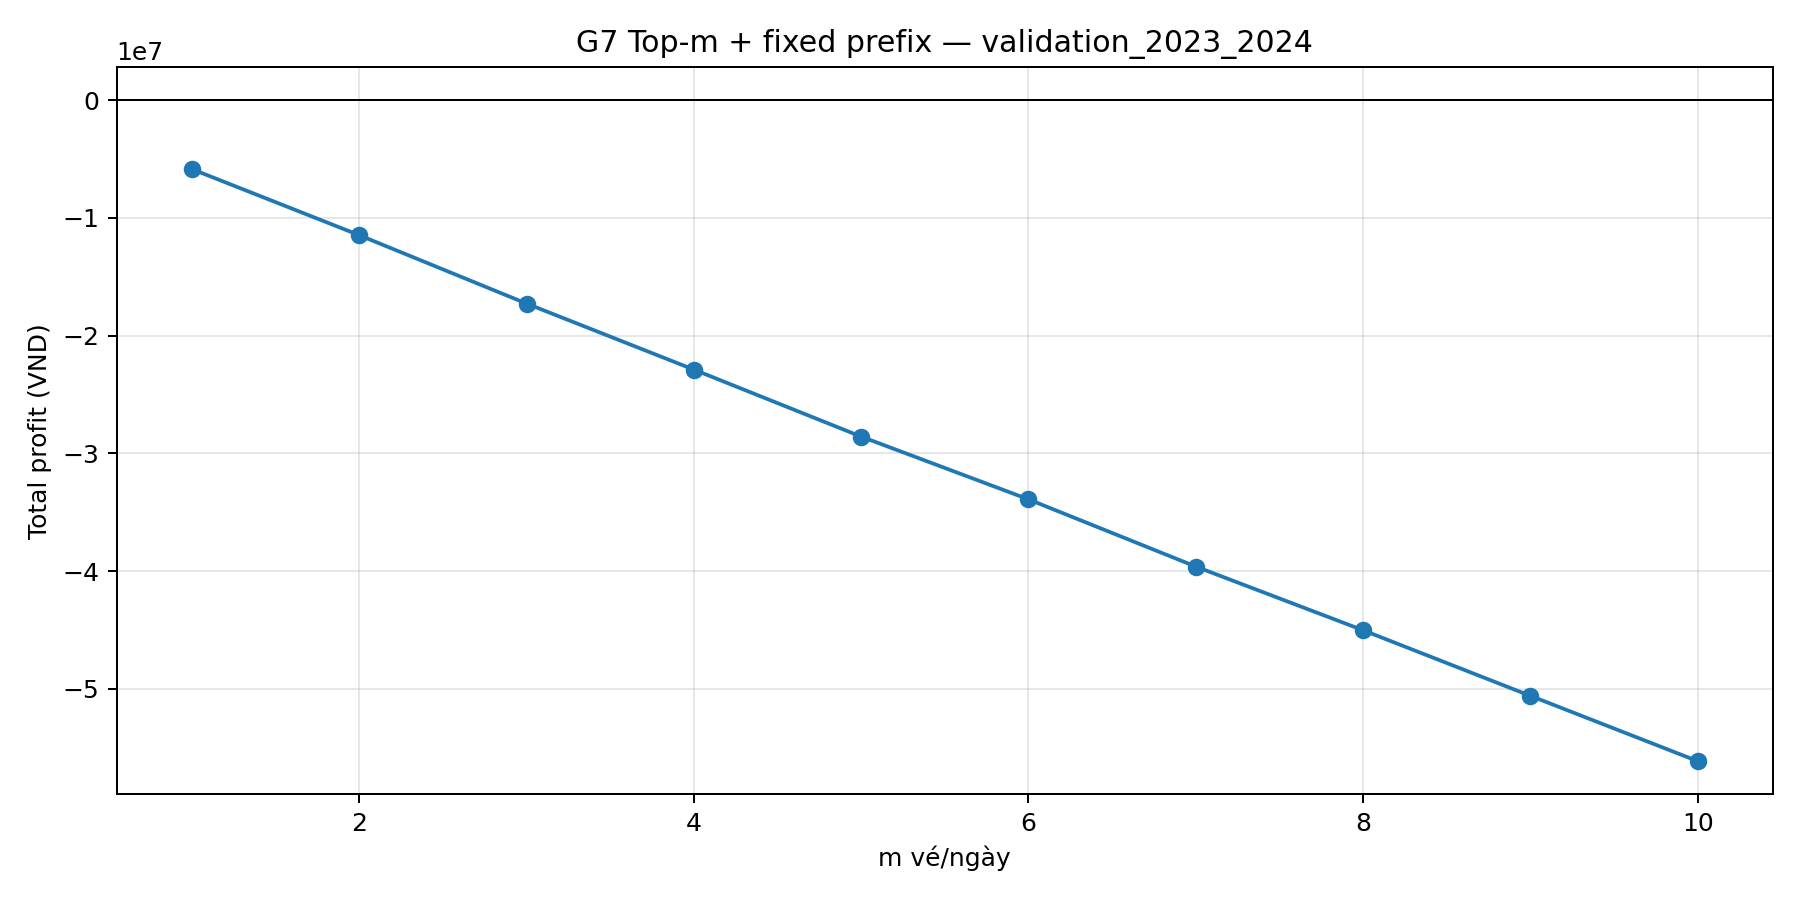
\includegraphics[width=0.92\linewidth]{../artifacts/p3_strategies/g7_topm_prefix/profit_by_m_validation_2023_2024.png}\caption{Độ nhạy lợi nhuận theo số đuôi $m$ trên validation.}\end{figure}
\begin{figure}[H]\centering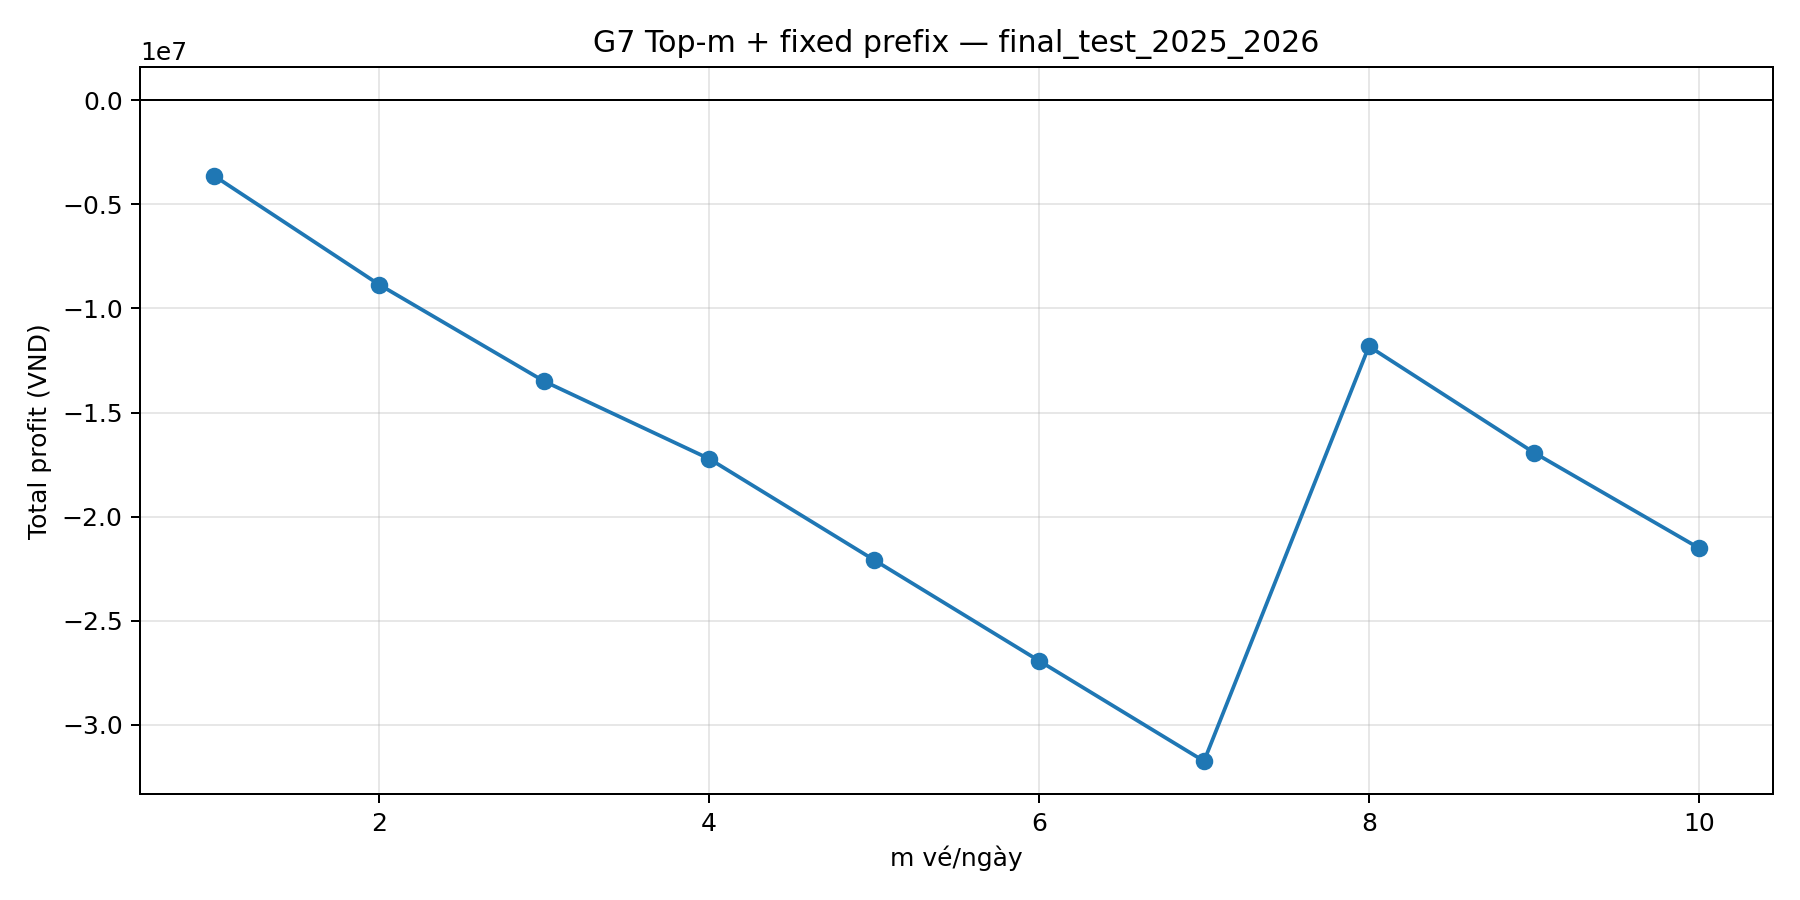
\includegraphics[width=0.92\linewidth]{../artifacts/p3_strategies/g7_topm_prefix/profit_by_m_final_test_2025_2026.png}\caption{Độ nhạy lợi nhuận theo số đuôi $m$ trên final test.}\end{figure}

\section{Diễn giải}
Tất cả cấu hình đều có ROI âm trên cả hai giai đoạn. Cấu hình 32 vé có tỷ lệ ngày có ít nhất một lần trúng cao hơn, nhưng chi phí cũng lớn hơn và tổng lợi nhuận vẫn âm. Đây là bằng chứng trực tiếp rằng một cải thiện nhỏ về thứ hạng chữ số trong P2 không chuyển thành lợi thế kinh tế trong cơ chế trả thưởng được mô phỏng.

\chapter{KẾT QUẢ TỔNG HỢP VÀ THẢO LUẬN}
\section{Từ kiểm định đến dự báo}
Phần 1 không tìm thấy phụ thuộc thời gian có hệ thống sau hiệu chỉnh nhiều kiểm định. Vì vậy, mô hình dự báo được xem là phép kiểm tra thực nghiệm về khả năng cải thiện ngoài mẫu, không phải giả định rằng dữ liệu chắc chắn có quy luật.

\section{So sánh mô hình}
Expanding Beta đứng đầu validation, trong khi CatBoost là mô hình học máy tốt nhất. Tuy nhiên chênh lệch giữa Expanding Beta và Uniform trên final test rất nhỏ. Top-$k$ cao ở $k$ lớn một phần do mục tiêu pool có độ phủ nhiều chữ số; không nên diễn giải như mô hình đã dự đoán chính xác một số năm chữ số.

Đối với mục tiêu giải, xác suất trúng một vé cụ thể nhỏ hơn rất nhiều so với xác suất một chữ số xuất hiện trong toàn bộ 27 giải. Vì vậy, báo cáo tách hai mục tiêu và chỉ sử dụng pool prediction để hỗ trợ sinh ứng viên, sau đó đánh giá trực tiếp vé theo kết quả thực tế và quy tắc trả thưởng.

\section{Ý nghĩa thực tiễn}
Lợi nhuận dương trong một giai đoạn không đủ chứng minh lợi thế dài hạn. Nếu kết quả không tái lập ở giai đoạn khác, kết luận phù hợp là hiệu năng chưa ổn định. Cần báo cáo khoảng tin cậy, nhiều giai đoạn rolling và số lần thử chiến lược.

\section{Hạn chế}
\begin{itemize}
\item Cách định nghĩa mục tiêu theo 27 kết quả ảnh hưởng mạnh đến độ khó.
\item Nhiều kiểm định và cấu hình làm tăng nguy cơ dương tính giả.
\item Final test chỉ phản ánh dữ liệu đã thu thập đến thời điểm báo cáo.
\item Lợi nhuận mẫu nhỏ có thể bị chi phối bởi một vài lần trúng.
\end{itemize}

\include{sections/07_ket_luan}

\backmatter
\fontsize{13pt}{18pt}\selectfont
\chapter*{TÀI LIỆU THAM KHẢO}\addcontentsline{toc}{chapter}{TÀI LIỆU THAM KHẢO}

[1] Benjamini, Y. and Hochberg, Y. (1995), Controlling the false discovery rate, JRSS Series B, 57(1), 289--300.
[2] Gelman, A. et al. (2013), Bayesian Data Analysis, 3rd ed., CRC Press.
[3] Bishop, C. M. (2006), Pattern Recognition and Machine Learning, Springer.
[4] Breiman, L. (2001), Random forests, Machine Learning, 45, 5--32.
[5] Chen, T. and Guestrin, C. (2016), XGBoost: A scalable tree boosting system, Proceedings of KDD.
[6] Prokhorenkova, L. et al. (2018), CatBoost: unbiased boosting with categorical features, NeurIPS.
[7] Gneiting, T. and Raftery, A. E. (2007), Strictly proper scoring rules, prediction, and estimation, JASA.
[8] Dawid, A. P. (1982), The well-calibrated Bayesian, JASA.
[9] Repository KQXS, nhánh lotery-update, GitHub, truy cập 09/2026.
[10] Repository template qh25-data-mining/report, GitHub, truy cập 09/2026.

\end{document}
